\documentclass[11pt,reqno]{amsart}
\usepackage{iftex}
\ifPDFTeX
  \usepackage[T1]{fontenc}
  \usepackage[utf8]{inputenc}
  \usepackage{lmodern}
\else
  \usepackage[no-math]{fontspec}
\fi
\usepackage{amsmath}
\usepackage{amssymb}
\usepackage{amsfonts}
\usepackage{mathrsfs}
\usepackage{amsthm}
\usepackage{mathtools}
\usepackage{geometry}
\usepackage{enumitem}
\usepackage{longtable}
\usepackage{booktabs}
\usepackage{array}
\usepackage{microtype}
\usepackage{graphicx}
\graphicspath{{../figures/}{figures/}}
\usepackage[dvipsnames]{xcolor}
\usepackage{float}
\usepackage{listings}
\lstset{basicstyle=\ttfamily\scriptsize,breaklines=true,columns=fullflexible,keepspaces=true,
  frame=single,framerule=0.3pt,showstringspaces=false,keywordstyle=\color{NavyBlue},
  commentstyle=\color{OliveGreen},stringstyle=\color{BrickRed},upquote=true}
\usepackage[pagebackref=true]{hyperref}
\usepackage{bookmark}
\usepackage{pdfcomment}

% Hover previews for internal references (no layout change).
\makeatletter
\let\CG@origref\ref
\let\CG@origeqref\eqref
\newcommand{\CG@gettip}[1]{\@ifundefined{CGTip@#1}{Reference: #1}{\csname CGTip@#1\endcsname}}
\DeclareRobustCommand{\CGref}[1]{\pdftooltip{\CG@origref{#1}}{\CG@gettip{#1}}}
\DeclareRobustCommand{\CGeqref}[1]{\pdftooltip{\CG@origeqref{#1}}{\CG@gettip{#1}}}
\makeatother
% Tooltip texts shown when hovering over internal references.
\makeatletter
\makeatother

\hypersetup{
  colorlinks=false,
  pdfborder={0 0 1},
  linkbordercolor={1 0 0},
  citebordercolor={0 0.3 1},
  urlbordercolor={0 0.6 0.6},
  filebordercolor={0 0.6 0.6},
  linktoc=all,
  bookmarksnumbered=true,
  bookmarksopen=true,
  bookmarksopenlevel=1,
  pdfstartview=FitH,
  pdftitle={Variable prime cutoffs in the Franca-LeClair equation and the prime phase of the Riemann zeros},
  pdfauthor={Rotkiv Ayn\"asac},
  pdfsubject={Riemann zeros, Franca-LeClair equation, truncated Euler products, ordinal-dependent prime cutoffs, exact identities at the zeros, prime phase of the displacement},
  pdfkeywords={Riemann zeta function, zeros, Lambert W clock, Franca-LeClair equation, Euler product, prime cutoff, argument of zeta, Selberg, Landau formula, pair correlation}
}
% Back-references in the bibliography (placed after the DOI).
\renewcommand*{\backref}[1]{}
\renewcommand*{\backrefalt}[4]{%
  \ifcase #1 %
    \relax
  \or
    \ (Cited on p.~#2.)%
  \else
    \ (Cited on pp.~#2.)%
  \fi}

% In \cite[note]{key} the note (e.g. a section number) is linked too.
\makeatletter
\let\CG@origcite\cite
\renewcommand*{\cite}[2][]{\def\CG@citekey{#2}%
  \ifx\relax#1\relax\CG@origcite{#2}\else\CG@origcite[#1]{#2}\fi}
\def\@cite#1#2{{\@citestyle[\citeform{#1}\if@tempswa, \hyper@link{cite}{cite.\CG@citekey}{#2}\fi]}}
\makeatother

\geometry{margin=1in}
\numberwithin{equation}{section}
\setcounter{tocdepth}{3}
\setcounter{secnumdepth}{3}
\setlength{\emergencystretch}{1.5em}

\theoremstyle{plain}
\newtheorem{theorem}{Theorem}[section]
\newtheorem{proposition}[theorem]{Proposition}
\newtheorem{lemma}[theorem]{Lemma}
\newtheorem{corollary}[theorem]{Corollary}
\newtheorem{conjecture}[theorem]{Conjecture}
\theoremstyle{definition}
\newtheorem{definition}[theorem]{Definition}
\newtheorem{hypothesis}[theorem]{Hypothesis}
\newtheorem{heuristic}[theorem]{Heuristic}
\newtheorem{experiment}[theorem]{Experiment}
\newtheorem{question}[theorem]{Question}
\theoremstyle{remark}
\newtheorem{remark}[theorem]{Remark}
\newtheorem{warning}[theorem]{Warning}

\newcommand{\R}{\mathbb R}
\newcommand{\NO}{N_0}
\newcommand{\lL}{\mathcal L}
\newcommand{\IT}{\mathcal I_T}
\newcommand{\sgn}{\operatorname{sgn}}
\newcommand{\mult}{\operatorname{mult}}
\newcommand{\Lan}{\mathfrak L}
\newcommand{\Gain}{\operatorname{Gain}}
\newcommand{\Diag}{\operatorname{Diag}}
\newcommand{\Exc}{\operatorname{Exc}}
\newcommand{\res}{\operatorname{res}}
\newcommand{\sk}{\mathsf k}
\providecommand{\NoCaseChange}[1]{\lowercase{#1}}

\begin{document}

\title[Variable prime cutoffs and the prime phase of the zeros]{Variable prime cutoffs in the Fran\c{c}a--LeClair equation\\ and the prime phase of the Riemann zeros}
\author{Rotkiv Ayn\"asac\\[2pt]{\normalfont\NoCaseChange{ROTKIVANYASAC@GMAIL.COM}}}
\date{16 October 2026 -- version 2}

\begin{abstract}
Let $\gamma_k$ be the positive ordinates of the zeros of $\zeta(s)$, counted with multiplicity, $\NO$ the smooth Riemann--von Mangoldt count, $s_k=k-\frac12-\NO(\gamma_k)$, and $S_X$ the argument of the Euler product over the primes $p\le X$. The paper contains four groups of results.
(i) Exact identities, with no hypothesis: for every $C^1$ counting model $F$, the sum of $(k-\frac12-F(\gamma_k))^2$ over consecutive zeros equals $\int(N-F)^2\,dF$ minus $\frac1{12}$ per zero plus explicit boundary terms; and $\sum_k s_kf(\gamma_k)$ is expressed exactly through $N-\NO$.
(ii) Unconditional estimates: uniformly for $2\le X\le T^{1/2}$, the mean of $u_k(X)^2=(s_k-S_X(\gamma_k))^2$ over $T<\gamma_k\le2T$ is $\frac1{2\pi^2}\log\frac{\log T}{\log X}+O(1+(\log\frac{\log T}{\log X})^{1/2})$. A fixed set of primes, as in LeClair's computations, leaves a defect of mean square $\sim\frac1{2\pi^2}\log\log T$; a cutoff $X=T^c$ keeps it bounded, and within $X\le T^{1/2}$ boundedness holds if and only if $\log X\asymp\log T$.
(iii) The prime phase $\Pi^\gamma_p=-2\pi\sqrt p\,\langle s_k\sin(\gamma_k\log p)\rangle$: unconditionally $\Pi^\gamma_p$ equals the Landau ratio of the zeros minus a multiple of the Fourier coefficient of $S(t)^2$ at frequency $\log p$; on the Riemann hypothesis the Landau ratio is $1+o(1)$ uniformly for $p\le T^{1-\eta}$. We conjecture $\Pi^\gamma_p\to1-(1+\theta)\log(1+\theta)-(1-\theta)\log(1-\theta)$ for $p=T^{\theta+o(1)}$, $0<\theta<1$, give a heuristic derivation in a GUE linear-response model with no free parameter, and an equivalent form for $\int S(t)^2p^{it}\,dt$.
(iv) Numerics on the first $2\,001\,052$ zeros and $2262$ primes: the conjectured law agrees with the data within the statistical error in five windows of height between $6\cdot10^3$ and $9\cdot10^5$.
\end{abstract}

\maketitle
\markboth{ROTKIV AYN\"ASAC}{VARIABLE PRIME CUTOFFS AND THE PRIME PHASE OF THE ZEROS}

\tableofcontents

\section{Introduction}
\label{sec:introduction}

Fran\c{c}a and LeClair \cite{FrancaLeClair2014,FrancaLeClair2015} proposed the equation
\begin{equation}
\NO(t)+\frac1\pi\lim_{\epsilon\to0^+}\arg\zeta\bigl(\tfrac12+\epsilon+it\bigr)=k-\frac12
\label{eq:intro_FL}
\end{equation}
for the ordinate of the $k$-th zero, where $\NO$ is the smooth part of the Riemann--von Mangoldt formula. Dropping the argument gives the Lambert-$W$ clock $\tau_k$. LeClair \cite{LeClair2021} replaces $\arg\zeta$ by the argument of an Euler product over $N_{\rm pr}$ primes, requires $N_{\rm pr}=N_{\rm pr}(t)\to\infty$ with $N_{\rm pr}<[t^2]$ \cite[Sect.~III]{LeClair2021}, supports the truncated equation by a random-walk model, and computes zeros near the ordinals $10^{21}$, $10^{22}$ and $10^{100}$ with the fixed value $N_{\rm pr}=5\times10^6$ \cite[Sect.~VI]{LeClair2021}.

This paper answers two questions about the truncated equation with proofs, and isolates a third phenomenon that we can state precisely but not prove.
\begin{enumerate}[label=(\Alph*),leftmargin=2em]
\item \emph{How well do the true zeros satisfy the truncated equation, and how must the number of primes depend on the height?} The defect $u_k(X)$ of Definition~\CGref{def:LeClair_model} has mean square $\frac1{2\pi^2}\log\frac{\log T}{\log X}+O(1+\sqrt{\cdot})$ uniformly for $2\le X\le T^{1/2}$ (Theorem~\CGref{thm:main}). The proof rests on an exact identity at the zeros (Theorem~\CGref{thm:identity_general}) and on Selberg's approximation of $S(t)$. Consequently a power cutoff $X=T^c$ is necessary and sufficient for a bounded mean-square defect (Corollary~\CGref{cor:dichotomy}); a fixed number of primes is not, and LeClair's growth condition $N_{\rm pr}\to\infty$ is not sufficient.
\item \emph{What does the Euler phase at a prime $p$ remove from the displacement?} The normalized projection $\Pi^\gamma_p$ of $s_k$ on $\sin(\gamma_k\log p)$ is expressed exactly through the Landau sum of the zeros and the Fourier coefficient of $S(t)^2$ at frequency $\log p$ (Proposition~\CGref{prop:phase_equivalence}); the Landau part is $1+o(1)$ on the Riemann hypothesis uniformly for $p\le T^{1-\eta}$ (Lemma~\CGref{lem:landau_ratio_RH}). The segment identity (Proposition~\CGref{prop:segment}) and an exact accounting of the one-step corrected clock (Proposition~\CGref{prop:accounting}) follow.
\item \emph{The prime phase law.} For $p=T^{\theta+o(1)}$ the data show a universal function of $\theta$. We conjecture (Conjecture~\CGref{conj:phase_law})
\begin{equation}
\Pi^\gamma_p\longrightarrow\Pi_*(\theta):=1-(1+\theta)\log(1+\theta)-(1-\theta)\log(1-\theta)=1-\theta^2-\frac{\theta^4}{6}-\cdots,
\label{eq:intro_law}
\end{equation}
derive it heuristically in a GUE linear-response model calibrated by Landau's formula (Appendix~\CGref{sec:appendix_model}), and show that it is equivalent, on the Riemann hypothesis, to an asymptotic formula for $\int_T^{2T}S(t)^2\cos(t\log p)\,dt$ (Proposition~\CGref{prop:conj_equivalent}). A proof would require information on the twisted pair correlation of the zeros outside the range accessible to Montgomery's method (Remark~\CGref{rem:twisted_status}).
\end{enumerate}

Three objects are kept apart throughout: the defect $u_k(X)$ of the true zero in the truncated equation, the solution $t_k^X$ of the truncated equation, and the residual $\res_k(X)$ of the one-step corrected clock, which is the quantity computed in the experiments.

\section{Notation}
\label{sec:notation}

All symbols used in the paper are listed here with their domains; no symbol is used with two meanings. Implied constants in $O(\cdot)$ and $\ll$ are absolute unless a subscript indicates a dependence. $\kappa_0,\kappa_1,\dots$ denote absolute positive constants.

\begin{center}
\small
\begin{longtable}{p{0.24\textwidth}p{0.70\textwidth}}
\toprule
symbol & meaning and domain\\
\midrule
\endfirsthead
\toprule
symbol & meaning and domain\\
\midrule
\endhead
$\rho=\beta+i\gamma$ & nontrivial zero of $\zeta$, $0<\beta<1$, $\gamma\in\R$\\
$\gamma_1\le\gamma_2\le\cdots$ & positive ordinates listed with multiplicity, $k\in\{1,2,\dots\}$\\
$\mult(\gamma)$ & multiplicity of an ordinate $\gamma$ (number of $k$ with $\gamma_k=\gamma$)\\
$N(t)$ & $\#\{k:\gamma_k\le t\}$, $t>0$; right continuous, nondecreasing\\
$\vartheta(t)$ & Riemann--Siegel theta function, $t>0$\\
$\Theta_0(t)$, $\varpi(t)$ & $\frac t2\log\frac t{2\pi e}-\frac\pi8$ and $\vartheta(t)-\Theta_0(t)$, $t>0$\\
$\NO(t)$, $\lL(t)$ & $\frac1\pi\Theta_0(t)+1$ and $\NO'(t)=\frac1{2\pi}\log\frac t{2\pi}$, $t>0$\\
$S(t)$, $S_1(t)$ & $\frac1\pi\arg\zeta(\frac12+it)$ for $t>0$ not an ordinate; $\int_0^tS$\\
$G(t)$ & $N(t)-\NO(t)$, $t>0$\\
$\tau_k$, $\tau(x)$ & clock: $\NO(\tau_k)=k-\frac12$; $\tau(x)$ the same for real $x\ge2$\\
$s_k$, $\delta_k$, $\xi_k$ & $k-\frac12-\NO(\gamma_k)$; $\tau_k-\gamma_k$; mean-value point between $\gamma_k$ and $\tau_k$\\
$T$, $\IT$, $k_\pm$ & height $T\ge T_0$; $\{k:T<\gamma_k\le2T\}$; smallest and largest element of $\IT$\\
$p$, $q$ & primes\\
$n$, $m$ & positive integers; $m$ is used as the exponent in $p^m$\\
$\Lambda(n)$, $\ell_n$ & von Mangoldt function; $\ell_n=\log n$\\
$a_n$ & $-\Lambda(n)/(\pi\sqrt n\log n)$ for $n\ge2$\\
$\mathcal A$, $S_{\mathcal A}$, $v_{\mathcal A}$ & set of prime powers; $\sum_{n\in\mathcal A}a_n\sin(t\ell_n)$; $\frac12\sum_{n\in\mathcal A}a_n^2$\\
$P$, $v^\infty_P$ & finite set of primes; $\frac1{2\pi^2}\sum_{p\in P}\mathrm{Li}_2(1/p)$\\
$X$, $c$ & prime cutoff, real $X\ge2$; $c=\log X/\log T$\\
$\mathcal A_X$, $S_X$ & $\{p^m:p\le X,m\ge1\}$; $S_{\mathcal A_X}$ (full local factors)\\
$U^{(0)}_X$, $U^{(1)}_X$ & bounds for $\sup|S_X|$ and $\sup|S_X'|$, \CGeqref{eq:U_def}\\
$F_X$, $u_k(X)$, $t_k^X$ & $\NO+S_X$; $k-\frac12-F_X(\gamma_k)$; solution of $F_X(t)=k-\frac12$\\
$\tau_k^X$, $\delta^X_k$, $\res_k(X)$ & one-step clock; $\tau^X_k-\gamma_k$; $\lL(\tau_k)\delta_k^X$\\
$\Omega$, $\mathrm{sat}_\Omega$ & saturation level $\Omega>0$; $y\mapsto\sgn(y)\min(|y|,\Omega)$\\
$\Phi_j$, $b_{j,r}$ & polynomials of Theorem~\CGref{thm:identity_general} and their coefficients\\
$\omega_j$, $\sigma_T$ & $\frac{(2j)!}{j!(2\pi)^{2j}}$; $\sigma_T^2=\frac1{2\pi^2}\log\log T$\\
$X_{\rm S}$, $S^{\rm pr}_{X_{\rm S}}$, $E_0$ & $T^{1/160}$; Selberg's prime polynomial; $S-S^{\rm pr}_{X_{\rm S}}$\\
$\Delta_X$, $D$, $\mathcal P^*$, $V$ & $S-S_X$; $S^{\rm pr}_{X_{\rm S}}-S_X$; primes between $X$ and $X_{\rm S}$; $\sum_{p\in\mathcal P^*}1/p$\\
$\theta_p$ & $\ell_p/\log(T/2\pi)$ for a prime $p$\\
$\Lan_n(T)$ & Landau ratio of the zeros, Definition~\CGref{def:landau_ratio}\\
$\Pi^\gamma_n$, $\Pi^\tau_n$, $\Pi_n(\nu)$ & prime phases at the zero, at the clock, on the segment, $\nu\in[0,1]$\\
$\Pi_*(\theta)$ & $1-(1+\theta)\log(1+\theta)-(1-\theta)\log(1-\theta)$, $0\le\theta<1$\\
$\Gain_{\mathcal A}$, $\Diag_{\mathcal A}$, $\Exc_{\mathcal A}$ & gain, diagonal gain and excess of the one-step clock, \CGeqref{eq:accounting_def}\\
$\eta$ & a fixed number in $(0,1)$\\
$K_*$ & $2\,001\,052$, number of zeros used in the experiments\\
$\sk$, $\mathsf R_r$, $\mathsf R^{\rm c}_r$, $\mathsf g$ & Appendix~\CGref{sec:appendix_model} only: sine kernel, correlation and cluster functions, potential amplitude\\
$\mathcal J$, $h_2$, $\mathfrak F_\theta$ & Appendices only: Hilbert part, binary entropy, twisted form factor\\
\bottomrule
\end{longtable}
\end{center}

\section{Standard results used}
\label{sec:known_results}

Nothing in this section is new.

\begin{theorem}[{\cite[Thms.~9.3, 9.4, 9.9 and \S9.4]{Titchmarsh1986}}, \cite{Littlewood1924}]\label{thm:known_basic}
For $t>0$ not an ordinate, $N(t)=\frac1\pi\vartheta(t)+1+S(t)$. There are absolute constants $\kappa_1,\kappa_2$ such that $|S(t)|\le\kappa_2\log t$ for $t\ge14$, every interval $[t,t+\kappa_1]$ with $t\ge14$ contains an ordinate, and $S_1(t)=O(\log t)$.
\end{theorem}

\begin{theorem}[Bellotti--Wong {\cite{BellottiWong2025}}]\label{thm:known_BW}
For $T\ge e$,
\begin{equation}
\Bigl|N(T)-\frac T{2\pi}\log\frac T{2\pi e}\Bigr|\le0.10076\log T+0.24460\log\log T+8.08344 .
\label{eq:BW_bound}
\end{equation}
\end{theorem}

\begin{theorem}[Selberg {\cite{Selberg1946a}}; as stated in {\cite[p.~225]{Fujii1974}}]\label{thm:known_selberg_moments}
For every integer $j\ge1$,
\begin{equation}
\int_T^{2T}S(t)^{2j}\,dt=\omega_jT(\log\log T)^j+O_j\bigl(T(\log\log T)^{j-1/2}\bigr).
\label{eq:selberg_moments}
\end{equation}
\end{theorem}

\begin{theorem}[Selberg's approximation in the form of {\cite[\S3, pp.~232--233]{Fujii1974}}; \cite{Selberg1946b}]\label{thm:known_selberg_approx}
Let $X_{\rm S}=T^{1/160}$ and $S^{\rm pr}_{X_{\rm S}}(t)=-\frac1\pi\sum_{p<X_{\rm S}}p^{-1/2}\sin(t\log p)$. Then $\int_T^{2T}(S-S^{\rm pr}_{X_{\rm S}})^4\,dt\le\kappa_3T$ for $T\ge T_0$.
\end{theorem}

\begin{proof}[Source of the statement]
In \cite[\S3]{Fujii1974}, $S(t,\chi)-\frac1\pi\Im\sum_{p<x^3}\chi(p)p^{-1/2-it}=\sum_{r=1}^5O(\mathcal B_r(t))$ with explicit functions $\mathcal B_r$, and on p.~233 it is shown that $(\int_T^{T+H}|\mathcal B_r|^{2j})^{1/2j}\ll j^2H^{1/2j}$ for $x=T^{a_2/60j}$ under the hypotheses of the Main Theorem there ($0<a_2\le\frac14$, modulus $\le T^{1/4-a_1}$, $T^{1/2+a_2}\le H\le T$). Take the principal character modulo $1$, $j=2$, $a_2=\frac14$, $H=T$; then $x^3=T^{1/160}$ and $\frac1\pi\Im p^{-1/2-it}=-\frac1\pi p^{-1/2}\sin(t\log p)$.
\end{proof}

\begin{theorem}[Montgomery--Vaughan {\cite[Cor.~3]{MontgomeryVaughan1974}}]\label{thm:known_MV}
For complex $w_n$, $\int_T^{2T}|\sum_{n\le Y}w_nn^{-it}|^2dt=\sum_{n\le Y}|w_n|^2(T+O(n))$.
\end{theorem}

\begin{theorem}[Mertens {\cite{Mertens1874}}]\label{thm:known_mertens}
For $2\le y_1\le y_2$, $\sum_{p\le y_2}\frac{\log p}p=\log y_2+O(1)$ and $\sum_{y_1<p\le y_2}\frac1p=\log\frac{\log y_2}{\log y_1}+O\bigl(\frac1{\log y_1}\bigr)$.
\end{theorem}

\begin{theorem}[Kusmin--Landau {\cite[Thm.~2.1]{GrahamKolesnik1991}}]\label{thm:known_KL}
Let $f$ be real with continuous monotone derivative on $[x_1,x_2]$ and $\|f'(x)\|\ge\lambda>0$ there, $\|\cdot\|$ the distance to the nearest integer. Then $|\sum_{x_1<k\le x_2}e^{2\pi if(k)}|\le\kappa_4\lambda^{-1}$.
\end{theorem}

\begin{theorem}[Landau {\cite{Landau1912}}; uniform version by Gonek {\cite{Gonek1993}}]\label{thm:known_landau}
For integers $n\ge2$ and $t>1$,
\begin{equation}
\sum_{0<\gamma\le t}n^{\rho}=-\frac t{2\pi}\Lambda(n)+O\bigl(n\log(2nt)\log\log(3n)\bigr),
\label{eq:landau_gonek}
\end{equation}
the zeros being counted with multiplicity.
\end{theorem}

\begin{theorem}[Littlewood; {\cite[Thm.~14.13]{Titchmarsh1986}}]\label{thm:known_RH_S}
On the Riemann hypothesis, $S(t)=O(\log t/\log\log t)$.
\end{theorem}

\section{The clock and the truncated equation}
\label{sec:clock}

\begin{lemma}\label{lem:clock}
For real $x\ge2$ put $\tau(x)=2\pi(x-\frac{11}8)/W((x-\frac{11}8)/e)$ with the principal branch of the Lambert function \cite{Corless1996}. Then $\tau(x)>2\pi$, $\tau(x)$ is the unique solution $t>2\pi$ of $\NO(t)=x-\frac12$, and $\tau'(x)=1/\lL(\tau(x))=2\pi/\log(\tau(x)/2\pi)$. We write $\tau_k=\tau(k)$.
\end{lemma}

\begin{proof}
Let $z=(x-\frac{11}8)/e>0$ and $t=2\pi(x-\frac{11}8)/W(z)$. Since $W(z)e^{W(z)}=z$, $t/(2\pi e)=z/W(z)=e^{W(z)}$, so $\log\frac t{2\pi e}=W(z)$ and $\frac t{2\pi}\log\frac t{2\pi e}=x-\frac{11}8$. By \CGeqref{eq:N0_def} this is $\NO(t)=x-\frac12$. Moreover $t/2\pi=e^{1+W(z)}>1$. On $(2\pi,\infty)$ the function $\NO$ has derivative $\lL>0$, which gives uniqueness and the formula for $\tau'$.
\end{proof}

Here and below
\begin{equation}
\Theta_0(t)=\frac t2\log\frac t{2\pi e}-\frac\pi8,\qquad\NO(t)=\frac1\pi\Theta_0(t)+1,\qquad\lL(t)=\frac1{2\pi}\log\frac t{2\pi},\qquad\varpi(t)=\vartheta(t)-\Theta_0(t),
\label{eq:N0_def}
\end{equation}
and Stirling's formula gives $\varpi(t)=\frac1{48t}+O(t^{-3})$, so $|\varpi(t)|\le\frac1{40t}$ for $t\ge T_0$. By Theorem~\CGref{thm:known_basic}, for $t>0$ not an ordinate,
\begin{equation}
G(t)=N(t)-\NO(t)=S(t)+\frac{\varpi(t)}\pi .
\label{eq:G_def}
\end{equation}

\begin{definition}\label{def:displacements}
For $k\ge2$, $s_k=k-\frac12-\NO(\gamma_k)$ and $\delta_k=\tau_k-\gamma_k$. By Lemma~\CGref{lem:clock}, $s_k=\NO(\tau_k)-\NO(\gamma_k)$, and the mean value theorem gives a point $\xi_k$ between $\gamma_k$ and $\tau_k$ with
\begin{equation}
s_k=\lL(\xi_k)\,\delta_k .
\label{eq:s_delta}
\end{equation}
\end{definition}

\begin{lemma}\label{lem:s_bounds}
For every $k$ with $\gamma_k\ge14$,
\begin{equation}
N(\gamma_k^-)-\NO(\gamma_k)+\frac12\le s_k\le N(\gamma_k^+)-\NO(\gamma_k)-\frac12,
\label{eq:s_bounds}
\end{equation}
and $|s_k|\le2\kappa_2\log\gamma_k+1$.
\end{lemma}

\begin{proof}
The indices $j$ with $\gamma_j=\gamma_k$ are $N(\gamma_k^-)+1,\dots,N(\gamma_k^+)$, so $N(\gamma_k^-)+1\le k\le N(\gamma_k^+)$; subtract $\frac12+\NO(\gamma_k)$. By \CGeqref{eq:G_def}, $N(\gamma_k^\pm)-\NO(\gamma_k)=S(\gamma_k^\pm)+\varpi(\gamma_k)/\pi$, and Theorem~\CGref{thm:known_basic} bounds both one-sided limits of $|S|$ by $\kappa_2\log\gamma_k$.
\end{proof}

For $n\ge2$ let $a_n=-\Lambda(n)/(\pi\sqrt n\log n)$. For real $X\ge2$ let $\mathcal A_X=\{p^m:p\le X,\ m\ge1\}$ and
\begin{equation}
S_X(t)=-\frac1\pi\sum_{p\le X}\arg\bigl(1-p^{-1/2-it}\bigr)=\sum_{n\in\mathcal A_X}a_n\sin(t\log n),
\label{eq:SX_def}
\end{equation}
with the principal argument; the series converges absolutely because $\arg(1-z)=-\Im\sum_{m\ge1}z^m/m$ for $|z|<1$. $S_X$ is a finite sum of real-analytic functions of $t$, and
\begin{equation}
|S_X(t)|\le U^{(0)}_X:=\frac1\pi\sum_{p\le X}\sum_{m\ge1}\frac1{m\,p^{m/2}},\qquad|S_X'(t)|\le U^{(1)}_X:=\frac1\pi\sum_{p\le X}\frac{\log p}{\sqrt p-1},
\label{eq:U_def}
\end{equation}
with $U^{(0)}_X\ll\sqrt X/\log X$ and $U^{(1)}_X\ll\sqrt X$ by Chebyshev's bound.

\begin{definition}\label{def:LeClair_model}
For $X\ge2$: $F_X=\NO+S_X$; the defect $u_k(X)=k-\frac12-F_X(\gamma_k)=s_k-S_X(\gamma_k)$; any solution $t_k^X$ of $F_X(t)=k-\frac12$ is a solution of the truncated equation; the one-step clock is $\tau_k^X=\tau_k-S_X(\tau_k)/\lL(\tau_k)$, with saturated version $\tau_k^{X,\Omega}=\tau_k-\mathrm{sat}_\Omega(S_X(\tau_k)/\lL(\tau_k))$; and $\delta^X_k=\tau^X_k-\gamma_k$, $\res_k(X)=\lL(\tau_k)\delta^X_k$.
\end{definition}

\begin{lemma}\label{lem:LeClair_equation}
Equation \CGeqref{eq:intro_FL} reads $\NO(t)+S(t)=k-\frac12$. Replacing $\arg\zeta(\frac12+it)$ by $\arg\prod_{p\le X}(1-p^{-1/2-it})^{-1}$ turns it into $F_X(t)=k-\frac12$, and $\tau^X_k$ is one step of $t\mapsto t-(F_X(t)-k+\frac12)/\lL(t)$ started at $\tau_k$.
\end{lemma}

\begin{proof}
The argument of the product is $-\sum_{p\le X}\arg(1-p^{-1/2-it})=\pi S_X(t)$, and $F_X(\tau_k)-k+\frac12=S_X(\tau_k)$ by Lemma~\CGref{lem:clock}.
\end{proof}

\section{Exact identities at the zeros}
\label{sec:identities}

We have not found the following identities in the literature consulted. They need no hypothesis on the zeros, not even simplicity.

\begin{theorem}\label{thm:identity_general}
Let $k_1<k_2$ be positive integers, let $F$ be a real function of class $C^1$ on $[\gamma_{k_1},\gamma_{k_2}]$ (one-sided derivatives at the end points), and put $u_k=k-\frac12-F(\gamma_k)$ for $k_1\le k\le k_2$. For every integer $j\ge1$ the integral below exists and
\begin{equation}
\int_{\gamma_{k_1}}^{\gamma_{k_2}}\bigl(N(t)-F(t)\bigr)^{2j}F'(t)\,dt=\sum_{k=k_1+1}^{k_2-1}\Phi_j(u_k)+\frac{(\frac12+u_{k_1})^{2j+1}+(\frac12-u_{k_2})^{2j+1}}{2j+1},
\label{eq:identity_general}
\end{equation}
where
\begin{equation}
\Phi_j(u)=\frac{(\frac12+u)^{2j+1}+(\frac12-u)^{2j+1}}{2j+1}=\sum_{r=0}^{j}b_{j,r}u^{2r},\qquad b_{j,r}=\binom{2j+1}{2r}\frac{2^{2r-2j}}{2j+1},\quad b_{j,j}=1 .
\label{eq:Phi_def}
\end{equation}
For $j=1$, $\Phi_1(u)=u^2+\frac1{12}$ and
\begin{equation}
\sum_{k=k_1+1}^{k_2-1}u_k^2=\int_{\gamma_{k_1}}^{\gamma_{k_2}}\bigl(N-F\bigr)^2F'\,dt-\frac{k_2-k_1-1}{12}-\frac{(\frac12+u_{k_1})^3+(\frac12-u_{k_2})^3}3 .
\label{eq:identity_quadratic}
\end{equation}
\end{theorem}

\begin{proof}
\emph{Existence.} $[\gamma_{k_1},\gamma_{k_2}]$ contains finitely many ordinates; between them $N$ is constant, so the integrand is bounded and continuous except at finitely many points, and the Riemann integral exists.

\emph{One gap.} Fix $k$ with $k_1\le k<k_2$. If $\gamma_k<\gamma_{k+1}$, then for $t\in(\gamma_k,\gamma_{k+1})$ exactly $k$ ordinates counted with multiplicity are $\le t$, so $N(t)=k$. The substitution $y=F(t)$, valid for every $C^1$ function whether monotone or not, gives
\begin{equation}
\int_{\gamma_k}^{\gamma_{k+1}}(k-F(t))^{2j}F'(t)\,dt=\int_{F(\gamma_k)}^{F(\gamma_{k+1})}(k-y)^{2j}dy=\frac{(\frac12-u_{k+1})^{2j+1}+(\frac12+u_k)^{2j+1}}{2j+1},
\label{eq:identity_one_gap}
\end{equation}
because $F(\gamma_k)-k=-\frac12-u_k$ and $F(\gamma_{k+1})-k=\frac12-u_{k+1}$. If $\gamma_k=\gamma_{k+1}$, the left side of \CGeqref{eq:identity_one_gap} vanishes; then $F(\gamma_{k+1})=F(\gamma_k)$, so $u_{k+1}=u_k+1$ and the right side equals $\frac{(-\frac12-u_k)^{2j+1}+(\frac12+u_k)^{2j+1}}{2j+1}=0$. Hence \CGeqref{eq:identity_one_gap} holds for every $k_1\le k<k_2$.

\emph{Summation.} The intervals $[\gamma_k,\gamma_{k+1}]$, $k_1\le k<k_2$, cover $[\gamma_{k_1},\gamma_{k_2}]$ and overlap only at end points. Summing \CGeqref{eq:identity_one_gap}, the term $(\frac12+u_k)^{2j+1}$ with $k_1<k<k_2$ pairs with $(\frac12-u_k)^{2j+1}$ from the gap ending at $\gamma_k$, which gives $\Phi_j(u_k)$; the unpaired terms are $(\frac12+u_{k_1})^{2j+1}$ and $(\frac12-u_{k_2})^{2j+1}$. The binomial expansion of $(\frac12+u)^{2j+1}+(\frac12-u)^{2j+1}$ keeps the even powers $u^{2r}$ with coefficient $2\binom{2j+1}{2r}2^{2r-2j-1}$, which gives \CGeqref{eq:Phi_def}; $b_{1,0}=\frac1{12}$, $b_{1,1}=1$.
\end{proof}

\begin{remark}\label{rem:twelfth}
Between consecutive distinct ordinates $N-F$ runs through one unit of the variable $y=F(t)$; the term $\frac1{12}$ is the mean square of this centred sawtooth.
\end{remark}

\begin{lemma}\label{lem:first_moment_identity}
Let $14\le t_1<t_2$ be points which are not ordinates and let $f$ be a real or complex function of class $C^1$ on $[t_1,t_2]$. Then
\begin{equation}
\sum_{t_1<\gamma_k\le t_2}s_kf(\gamma_k)=\int_{t_1}^{t_2}G(t)f(t)\lL(t)\,dt+\frac12\Bigl[fG^2\Bigr]_{t_1}^{t_2}-\frac12\int_{t_1}^{t_2}G(t)^2f'(t)\,dt .
\label{eq:first_moment_identity}
\end{equation}
\end{lemma}

\begin{proof}
Let $\gamma^{(1)}<\dots<\gamma^{(R)}$ be the distinct ordinates in $(t_1,t_2]$; $R<\infty$. Put $G^*(\gamma)=\frac12(G(\gamma^-)+G(\gamma^+))$; then $G(\gamma^+)-G(\gamma^-)=\mult(\gamma)$.

\emph{Left side.} The indices with $\gamma_k=\gamma$ are $N(\gamma^-)+1,\dots,N(\gamma^-)+\mult(\gamma)$, so $\sum_{\gamma_k=\gamma}(k-\frac12)=\mult(\gamma)N(\gamma^-)+\frac12\mult(\gamma)^2=\mult(\gamma)\frac{N(\gamma^-)+N(\gamma^+)}2$, and since $\NO$ is continuous, $\sum_{\gamma_k=\gamma}s_k=\mult(\gamma)G^*(\gamma)$. Hence the left side is $\sum_{r=1}^R\mult(\gamma^{(r)})f(\gamma^{(r)})G^*(\gamma^{(r)})$.

\emph{Right side.} Put $\gamma^{(0)}=t_1$, $\gamma^{(R+1)}=t_2$. On each open interval $(\gamma^{(r)},\gamma^{(r+1)})$ the function $G$ is $C^1$ with $G'=-\lL$, so $(fG^2)'=f'G^2-2fG\lL$. Integrating over each interval and adding the jumps of $fG^2$ at the ordinates,
\begin{equation}
\Bigl[fG^2\Bigr]_{t_1}^{t_2}=\int_{t_1}^{t_2}\bigl(f'G^2-2fG\lL\bigr)dt+\sum_{r=1}^Rf(\gamma^{(r)})\bigl(G(\gamma^{(r)+})^2-G(\gamma^{(r)-})^2\bigr).
\label{eq:first_moment_telescoping}
\end{equation}
The jump equals $(G(\gamma^+)-G(\gamma^-))(G(\gamma^+)+G(\gamma^-))=2\mult(\gamma)G^*(\gamma)$. Solving \CGeqref{eq:first_moment_telescoping} for the sum of the jumps gives \CGeqref{eq:first_moment_identity}.
\end{proof}

\begin{corollary}\label{cor:cumulative}
$\sum_{\gamma_k\le t}s_k=O(\log^2t)$ for $t\ge14$ not an ordinate.
\end{corollary}

\begin{proof}
Lemma~\CGref{lem:first_moment_identity} with $f\equiv1$, $t_1=14<\gamma_1$, $t_2=t$: $|G|\ll\log t$, and by \CGeqref{eq:G_def} and integration by parts, $\int_{14}^tG\lL\,du=\lL(t)(S_1(t)-S_1(14))-\int_{14}^t(S_1(u)-S_1(14))\frac{du}{2\pi u}+O(\log t)=O(\log^2t)$ by $S_1=O(\log t)$.
\end{proof}

\section{Moments and extremes of the clock displacement}
\label{sec:clock_moments}

Throughout, $T\ge T_0$ and $T$, $2T$ are not ordinates; $k_-$ and $k_+$ are the smallest and largest indices in $\IT$. By Theorem~\CGref{thm:known_basic}, $\gamma_{k_-}-T\le\kappa_1$ and $2T-\gamma_{k_+}\le\kappa_1$, and
\begin{equation}
\#\IT=N(2T)-N(T)=\int_T^{2T}\lL\,dt+O(\log T)=T\lL(T)+O(T),
\label{eq:IT_size}
\end{equation}
because $0\le\lL(t)-\lL(T)\le\frac{\log2}{2\pi}$ on $[T,2T]$.

\begin{theorem}\label{thm:clock_moments}
For every integer $j\ge1$,
\begin{equation}
\frac1{\#\IT}\sum_{k\in\IT}s_k^{2j}=\omega_j(\log\log T)^j+O_j\bigl((\log\log T)^{j-1/2}\bigr).
\label{eq:clock_moments}
\end{equation}
\end{theorem}

\begin{proof}
Apply Theorem~\CGref{thm:identity_general} with $F=\NO$, $k_1=k_-$, $k_2=k_+$; then $u_k=s_k$ and $N-\NO=G$. By Lemma~\CGref{lem:s_bounds}, $|s_k|\le2\kappa_2\log(2T)+1$ for $k\in\IT$, so the two boundary terms of \CGeqref{eq:identity_general} and $\Phi_j(s_{k_\pm})$ are $O_j(\log^{2j+1}T)$. On $[T,\gamma_{k_-}]\cup[\gamma_{k_+},2T]$, of total length $\le2\kappa_1$, the integrand is $O_j(\log^{2j+1}T)$; so
\begin{equation}
\sum_{k\in\IT}\Phi_j(s_k)=\int_T^{2T}G^{2j}\lL\,dt+O_j(\log^{2j+1}T).
\label{eq:moments_step1}
\end{equation}
By \CGeqref{eq:G_def}, $|G^{2j}-S^{2j}|\le2j\frac{|\varpi|}\pi(|S|+1)^{2j-1}\ll_jT^{-1}\log^{2j-1}T$, which contributes $O_j(\log^{2j}T)$. Since $\lL(t)=\lL(T)+O(1)$ on $[T,2T]$, Theorem~\CGref{thm:known_selberg_moments} gives
\begin{equation}
\int_T^{2T}S^{2j}\lL\,dt=\lL(T)\,\omega_jT(\log\log T)^j+O_j\bigl(\lL(T)\,T(\log\log T)^{j-1/2}\bigr).
\label{eq:moments_step2}
\end{equation}
Dividing by \CGeqref{eq:IT_size},
\begin{equation}
\frac1{\#\IT}\sum_{k\in\IT}\Phi_j(s_k)=\omega_j(\log\log T)^j+O_j\bigl((\log\log T)^{j-1/2}\bigr).
\label{eq:moments_step3}
\end{equation}
For $j=1$ this is \CGeqref{eq:clock_moments}, because $\Phi_1(s)=s^2+\frac1{12}$. If \CGeqref{eq:clock_moments} holds for all orders $r<j$, then $\frac1{\#\IT}\sum_{k}\sum_{r<j}b_{j,r}s_k^{2r}=O_j((\log\log T)^{j-1})$, and \CGeqref{eq:moments_step3} gives \CGeqref{eq:clock_moments} for $j$.
\end{proof}

\begin{corollary}\label{cor:clock_distribution}
For every fixed $\eta'\ge0$, $\frac1{\#\IT}\#\{k\in\IT:|s_k|\le\eta'\sigma_T\}\to\mathbb P(|Z|\le\eta')$, $Z$ standard normal. In particular $\#\{k\in\IT:|s_k|\le A'\}=o(\#\IT)$ for every fixed $A'>0$. Moreover $\frac1{\#\IT}\sum_{k\in\IT}\delta_k^2=\frac{2\log\log T}{\log^2T}(1+O((\log\log T)^{-1/2}))$.
\end{corollary}

\begin{proof}
By Theorem~\CGref{thm:clock_moments} the moments of $s_k^2/\sigma_T^2$ tend to $\omega_j(2\pi^2)^j=\frac{(2j)!}{j!2^j}=\mathbb E[Z^{2j}]$; the law of $Z^2$ is determined by its moments (its moment generating function is finite near $0$), and the method of moments \cite[\S30]{Billingsley1995} gives the first statement. For the last one use \CGeqref{eq:s_delta}, $|\delta_k|\ll1$ and $\lL(\xi_k)=\frac1{2\pi}\log T\,(1+O(1/\log T))$.
\end{proof}

\begin{remark}\label{rem:korolev_kargin}
Kargin proved that the normalized deviations of the zeros from their predicted positions are asymptotically Gaussian \cite{Kargin2013}, and Selberg stated and Korolev proved moment formulae for the integer displacement of $\gamma_n$ from the Gram intervals \cite{Korolev2012}. Theorem~\CGref{thm:clock_moments} is the corresponding statement for $s_k$; its proof is a consequence of Theorem~\CGref{thm:identity_general}. The clock point satisfies $\Theta_0(\tau_k)=\pi(k-\frac32)$, so $\tau_k$ lies in phase half way between the Gram points $g_{k-2}$ and $g_{k-1}$.
\end{remark}

\begin{proposition}\label{prop:extremes}
\textup{(a)} $\limsup_ks_k=+\infty$ and $\liminf_ks_k=-\infty$. \textup{(b)} $\limsup_k|\delta_k|\le2\pi\cdot0.10076=0.633093\ldots$. \textup{(c)} On the Riemann hypothesis $\delta_k\to0$. \textup{(d)} For fixed $X\ge2$ and $\Omega\in(0,\infty]$, $\limsup_k|\delta^{X,\Omega}_k|=\limsup_k|\delta_k|$ and $\limsup_k|u_k(X)|=\infty$.
\end{proposition}

\begin{proof}
(a) Let $\gamma_k<\gamma_{k+1}$ and $t\in(\gamma_k,\gamma_{k+1})$. Then $N(t)=k$ and $\NO(\gamma_k)\le\NO(t)\le\NO(\gamma_{k+1})$, so
\begin{equation}
s_{k+1}-\frac12\le G(t)\le s_k+\frac12 .
\label{eq:sawtooth_sandwich}
\end{equation}
Suppose $s_k\le A'$ for all $k\ge k_0$. Then $S\le A'+1$ on $[t_0,\infty)$ for some $t_0$, by \CGeqref{eq:G_def}. Since $\int_T^{2T}S\,dt=S_1(2T)-S_1(T)=O(\log T)$, $\int_T^{2T}S^-dt=\int_T^{2T}S^+dt-\int_T^{2T}S\,dt\le(A'+1)T+O(\log T)$, so $\int_T^{2T}|S|\le2(A'+1)T+O(\log T)$. Hölder's inequality with exponents $\frac32,3$ and \CGeqref{eq:selberg_moments} with $j=2$ give
\begin{equation}
\int_T^{2T}S^2\le\Bigl(\int_T^{2T}|S|\Bigr)^{2/3}\Bigl(\int_T^{2T}S^4\Bigr)^{1/3}\ll_{A'}T(\log\log T)^{2/3},
\label{eq:holder_contradiction}
\end{equation}
contradicting \CGeqref{eq:selberg_moments} with $j=1$. The statement for $\liminf$ follows in the same way from the left inequality of \CGeqref{eq:sawtooth_sandwich}.

(b) By Lemma~\CGref{lem:s_bounds} and \CGeqref{eq:BW_bound}, with $\NO(t)=\frac t{2\pi}\log\frac t{2\pi e}+\frac78$, $|s_k|\le0.10076\log\gamma_k+O(\log\log\gamma_k)$, and $|\delta_k|=|s_k|/\lL(\xi_k)$ with $\lL(\xi_k)=\frac1{2\pi}\log\gamma_k(1+o(1))$.

(c) Theorem~\CGref{thm:known_RH_S} and Lemma~\CGref{lem:s_bounds} give $s_k=O(\log\gamma_k/\log\log\gamma_k)$, hence $\delta_k=O(1/\log\log\gamma_k)$.

(d) $|\delta^{X,\Omega}_k-\delta_k|\le U^{(0)}_X/\lL(\tau_k)\to0$ and $|u_k(X)-s_k|\le U^{(0)}_X$; apply (a).
\end{proof}

\section{The main theorem: the defect in the truncated equation}
\label{sec:main_theorem}

\begin{theorem}\label{thm:main}
There are absolute constants $T_0$ and $\kappa_0$ such that for every $T\ge T_0$ and every real $X$ with $2\le X\le T^{1/2}$, writing $c=\log X/\log T\in(0,\frac12]$,
\begin{equation}
\Bigl|\frac1{\#\IT}\sum_{k\in\IT}u_k(X)^2-\frac1{2\pi^2}\log\frac1c\Bigr|\le\kappa_0\Bigl(1+\sqrt{\log(1/c)}\Bigr).
\label{eq:main_theorem}
\end{equation}
\end{theorem}

This is a uniform main-term estimate. It is asymptotic only when $\log(1/c)=\log\log T-\log\log X\to\infty$; for fixed $c$ both sides are $O(1)$ and the constant term is not determined (Question~\CGref{q:constant}). The theorem concerns the defect of the true zero; it says nothing about the location of solutions $t_k^X$ of the truncated equation, which need not be unique when $F_X$ is not monotone (Proposition~\CGref{prop:localization}).

\begin{corollary}\label{cor:fixed_cutoff}
For fixed $X\ge2$: $\frac1{\#\IT}\sum_{k\in\IT}u_k(X)^2=\frac1{2\pi^2}\log\log T+O_X(\sqrt{\log\log T})$, and $\#\{k\in\IT:|u_k(X)|\le A'\}=o(\#\IT)$ for every fixed $A'$.
\end{corollary}

\begin{proof}
The first claim is \CGeqref{eq:main_theorem}. For the second, $|u_k(X)-s_k|\le U^{(0)}_X$; apply Corollary~\CGref{cor:clock_distribution}.
\end{proof}

\begin{corollary}\label{cor:dichotomy}
Let $X=X(T)$ with $2\le X\le T^{1/2}$. The mean of $u_k(X)^2$ over $\IT$ is bounded as $T\to\infty$ if and only if $\liminf_{T\to\infty}\log X/\log T>0$. For fixed $X_*\ge2$ and fixed $c\in(0,\frac12]$,
\begin{equation}
\frac1{\#\IT}\sum_{k\in\IT}\bigl(u_k(X_*)^2-u_k(T^c)^2\bigr)=\frac1{2\pi^2}\log\log T+O_{X_*,c}\bigl(\sqrt{\log\log T}\bigr).
\label{eq:dichotomy}
\end{equation}
The same holds for $X=K^c$ with $K=N(T)$ and fixed $0<c<\frac12$, since then $X=T^{c_T}$ with $c_T=c+O(\log\log T/\log T)<\frac12$.
\end{corollary}

\begin{proof}
Both directions follow from \CGeqref{eq:main_theorem} because $y\mapsto\frac y{2\pi^2}-\kappa_0(1+\sqrt y)$ tends to $+\infty$; \CGeqref{eq:dichotomy} is the difference of the two cases of \CGeqref{eq:main_theorem}.
\end{proof}

\begin{remark}\label{rem:comparison_LeClair}
With $N_{\rm pr}=\#\{p\le X\}$ one has $\log N_{\rm pr}=\log X+O(\log\log X)$. Corollary~\CGref{cor:dichotomy} says that the truncated equation is satisfied by the zeros with bounded mean-square defect exactly when $\log N_{\rm pr}\asymp\log T$; a fixed $N_{\rm pr}$, as in \cite[Sect.~VI]{LeClair2021}, leaves a defect of mean square $\sim\frac1{2\pi^2}\log\log T$, and $N_{\rm pr}\to\infty$ with $\log N_{\rm pr}=o(\log T)$ does not suffice. LeClair's range $\frac12<c\le2$ is not covered (Question~\CGref{q:large_c}).
\end{remark}

\subsection{Lemmas on prime polynomials}
\label{subsec:main_lemmas}

Fix $T\ge T_0$ with $X_{\rm S}=T^{1/160}\ge2$ and $2\le X\le T^{1/2}$. Write $S_X=S^{(1)}_X+S^{(2)}_X+S^{(\ge3)}_X$ according to $m=1$, $m=2$, $m\ge3$ in \CGeqref{eq:SX_def}. Let $\mathcal P^*$ be the set of primes in $(X,X_{\rm S})$ if $X<X_{\rm S}$ and in $[X_{\rm S},X]$ otherwise, $\epsilon_*=+1$ in the first case and $-1$ in the second, and
\begin{equation}
D_1(t)=-\frac1\pi\sum_{p\in\mathcal P^*}\frac{\sin(t\log p)}{\sqrt p},\qquad V=\sum_{p\in\mathcal P^*}\frac1p,\qquad D=S^{\rm pr}_{X_{\rm S}}-S_X=\epsilon_*D_1-S^{(2)}_X-S^{(\ge3)}_X .
\label{eq:D_def}
\end{equation}

\begin{lemma}\label{lem:V_size}
$V=\log(1/c)+O(1)$, uniformly in $c\in(0,\frac12]$.
\end{lemma}

\begin{proof}
By Theorem~\CGref{thm:known_mertens}, $V=|\log\frac{\log X_{\rm S}}{\log X}|+O(1)=|\log\frac1{160c}|+O(1)$. If $c\le\frac1{160}$ this is $\log\frac1c-\log160+O(1)$; if $\frac1{160}<c\le\frac12$, both $V$ and $\log\frac1c$ are $O(1)$.
\end{proof}

\begin{lemma}\label{lem:trig_MV}
For real $w_n$, $2\le n\le Y$,
\begin{equation}
\int_T^{2T}\Bigl(\sum_{n\le Y}w_n\sin(t\log n)\Bigr)^2dt=\frac T2\sum_{n\le Y}w_n^2+O\Bigl(\sum_{n\le Y}nw_n^2+\Bigl(\sum_{n\le Y}|w_n|\Bigr)^2\Bigr),
\label{eq:trig_MV}
\end{equation}
and the same with $\cos$ in place of $\sin$.
\end{lemma}

\begin{proof}
With $Q(t)=\sum w_nn^{-it}$, $\sum w_n\sin(t\log n)=-\Im Q$ and $(\Im Q)^2=\frac12(|Q|^2-\Re Q^2)$. Theorem~\CGref{thm:known_MV} gives $\int|Q|^2$; and $|\int_T^{2T}(n_1n_2)^{-it}dt|\le2/\log(n_1n_2)\le2/\log4$ gives $|\int Q^2|\le\frac2{\log4}(\sum|w_n|)^2$. For $\cos$ use $\Re Q$.
\end{proof}

\begin{lemma}\label{lem:D_moments}
With absolute implied constants,
\begin{align}
\int_T^{2T}D^2\,dt&=\frac T{2\pi^2}V+O\bigl(T(1+\sqrt V)\bigr),
\label{eq:D_second}\\
\int_T^{2T}D^4\,dt&\ll T(1+V)^2,
\label{eq:D_fourth}\\
\int_T^{2T}S_X'^2\,dt&\ll T(1+\log X)^2 .
\label{eq:SX_derivative}
\end{align}
\end{lemma}

\begin{proof}
All primes involved are $\le\max(X,X_{\rm S})\le T^{1/2}$.

\eqref{eq:D_second}: Lemma~\CGref{lem:trig_MV} with $w_p=\frac1{\pi\sqrt p}$ gives $\int D_1^2=\frac T{2\pi^2}V+O(T^{1/2})$, since $\sum_{p\le T^{1/2}}1\le T^{1/2}$ and $(\sum_{p\le T^{1/2}}p^{-1/2})^2\le4T^{1/2}$. For $S^{(2)}_X(t)=-\frac1{2\pi}\sum_{p\le X}p^{-1}\sin(t\log p^2)$ the same lemma gives $\int(S^{(2)}_X)^2\ll T\sum p^{-2}+\#\{p\le X\}+(\sum_{p\le X}p^{-1})^2\ll T$. Finally $|S^{(\ge3)}_X|\le\frac1\pi\sum_p\sum_{m\ge3}\frac1{mp^{m/2}}\le\kappa_5$. Expanding $D^2$ and bounding the cross terms by the Cauchy--Schwarz inequality gives \CGeqref{eq:D_second}.

\eqref{eq:D_fourth}: $(y_1+y_2+y_3)^4\le27(y_1^4+y_2^4+y_3^4)$. Let $Q(t)=\sum_{p\in\mathcal P^*}p^{-1/2}p^{-it}$, so $|D_1|\le|Q|/\pi$ and $Q^2=\sum_nd_nn^{-it}$ with $d_{p^2}=p^{-1}$, $d_{pq}=2(pq)^{-1/2}$ for $p<q$, other $d_n=0$, and $n\le T$. Theorem~\CGref{thm:known_MV} gives $\int|Q|^4=\sum|d_n|^2(T+O(n))\ll T\sum|d_n|^2\le T(1+2V^2)$. For $S^{(2)}_X$, $|S^{(2)}_X|\le|Q_2|/2\pi$ with $Q_2(t)=\sum_{p\le X}p^{-1}(p^2)^{-it}$, and $Q_2^2=\sum_nd^{(2)}_nn^{-it}$ is supported on $n=(pq)^2\le X^4\le T^2$ with $|d^{(2)}_n|\le2(pq)^{-1}$; so $\sum|d^{(2)}_n|^2\ll1$ and $\sum n|d^{(2)}_n|^2\le4\#\{p\le X\}^2\le4X^2\le4T$. $S^{(\ge3)}_X$ is bounded by $\kappa_5$.

\eqref{eq:SX_derivative}: $S_X'(t)=\sum_{n\in\mathcal A_X}a_n\log n\cos(t\log n)$. The terms $m=1$ have coefficients $\frac{\log p}{\pi\sqrt p}$; Lemma~\CGref{lem:trig_MV} and Theorem~\CGref{thm:known_mertens} give $\ll T\log X\sum_{p\le X}\frac{\log p}p+\sum_{p\le X}\log^2p+(\sum_{p\le X}\frac{\log p}{\sqrt p})^2\ll T(1+\log X)^2+X\log^2X$, and $X\le T^{1/2}$. The terms $m=2$ have coefficients $\frac{\log p}{\pi p}$ and contribute $\ll T+X\log X+\log^2X$. The terms $m\ge3$ are bounded by $\frac1\pi\sum_p\sum_{m\ge3}p^{-m/2}\log p<\infty$.
\end{proof}

\subsection{Proof of the main theorem}
\label{subsec:main_proof}

Let $E_0=S-S^{\rm pr}_{X_{\rm S}}$ and $\Delta_X=S-S_X=E_0+D$. By Theorem~\CGref{thm:known_selberg_approx} and Hölder's inequality on an interval of length $T$,
\begin{equation}
\int_T^{2T}E_0^4\,dt\le\kappa_3T,\qquad\int_T^{2T}E_0^2\,dt\le T^{1/2}\Bigl(\int_T^{2T}E_0^4\Bigr)^{1/2}\le\kappa_3^{1/2}T .
\label{eq:E0_bounds}
\end{equation}
Let $J=\int_T^{2T}\Delta_X^2\,dt$. By \CGeqref{eq:D_second}, \CGeqref{eq:E0_bounds} and the Cauchy--Schwarz inequality,
\begin{equation}
J=\frac T{2\pi^2}V+O\bigl(T(1+\sqrt V)\bigr),
\label{eq:J_asymptotic}
\end{equation}
and by \CGeqref{eq:D_fourth}, \CGeqref{eq:E0_bounds} and $(y_1+y_2)^4\le8(y_1^4+y_2^4)$,
\begin{equation}
\int_T^{2T}\Delta_X^4\,dt\ll T(1+V)^2 .
\label{eq:R_fourth}
\end{equation}

\emph{Application of the identity.} $F_X$ is real-analytic on $(0,\infty)$. Theorem~\CGref{thm:identity_general} with $F=F_X$, $j=1$, $k_1=k_-$, $k_2=k_+$, and $N-F_X=\Delta_X+\varpi/\pi$ (from \CGeqref{eq:G_def}) give
\begin{equation}
\sum_{k=k_-+1}^{k_+-1}u_k(X)^2=\int_{\gamma_{k_-}}^{\gamma_{k_+}}\Bigl(\Delta_X+\frac\varpi\pi\Bigr)^2\bigl(\lL+S_X'\bigr)dt-\frac{k_+-k_--1}{12}-\frac{(\frac12+u_{k_-})^3+(\frac12-u_{k_+})^3}3 .
\label{eq:main_identity_applied}
\end{equation}

\emph{Boundary terms.} By Lemma~\CGref{lem:s_bounds} and \CGeqref{eq:U_def}, $|u_k(X)|\le2\kappa_2\log(2T)+1+U^{(0)}_X\ll\log T+\sqrt X\ll T^{1/4}$ for $k\in\IT$. Hence the last term of \CGeqref{eq:main_identity_applied} and $u_{k_\pm}(X)^2$ are $O(T^{3/4})$.

\emph{Edge intervals.} On $[T,\gamma_{k_-}]\cup[\gamma_{k_+},2T]$, of length $\le2\kappa_1$, $|\Delta_X|\ll\log T+\sqrt X$ and $\lL+|S_X'|\ll\log T+\sqrt X$, so the integrand is $O(T^{3/4})$.

\emph{The term $\varpi$.} Since $|\varpi|\le\frac1{40T}$ on $[T,2T]$, replacing $(\Delta_X+\varpi/\pi)^2$ by $\Delta_X^2$ costs at most $\frac1T\int_T^{2T}(|\Delta_X|+1)(\lL+|S_X'|)\,dt\ll(1+V)^{1/2}\log T$, by the Cauchy--Schwarz inequality, \CGeqref{eq:J_asymptotic} and \CGeqref{eq:SX_derivative}.

Therefore
\begin{equation}
\sum_{k\in\IT}u_k(X)^2=\int_T^{2T}\Delta_X^2\lL\,dt+\int_T^{2T}\Delta_X^2S_X'\,dt-\frac{\#\IT}{12}+O(T^{3/4}).
\label{eq:main_step1}
\end{equation}
The first integral is $\lL(T)J+O(J)$. By the Cauchy--Schwarz inequality, \CGeqref{eq:R_fourth} and \CGeqref{eq:SX_derivative},
\begin{equation}
\Bigl|\int_T^{2T}\Delta_X^2S_X'\,dt\Bigr|\le\Bigl(\int_T^{2T}\Delta_X^4\Bigr)^{1/2}\Bigl(\int_T^{2T}S_X'^2\Bigr)^{1/2}\ll T(1+V)(1+\log X).
\label{eq:main_step2}
\end{equation}
Dividing by $\#\IT=T\lL(T)+O(T)$ and using \CGeqref{eq:J_asymptotic},
\begin{equation}
\frac1{\#\IT}\sum_{k\in\IT}u_k(X)^2=\frac V{2\pi^2}+O\Bigl(1+\sqrt V+\frac{1+V}{\log T}+(1+V)\,c\Bigr),
\label{eq:main_step3}
\end{equation}
because $\log X=c\log T$. By Lemma~\CGref{lem:V_size}, $(1+V)c\ll c(1+\log\frac1c)\ll1$ for $0<c\le\frac12$; and $c\ge\log2/\log T$ gives $V\ll\log\log T$, so $(1+V)/\log T=o(1)$. A second application of Lemma~\CGref{lem:V_size} replaces $\frac V{2\pi^2}$ by $\frac1{2\pi^2}\log\frac1c+O(1)$ and $\sqrt V$ by $\sqrt{\log(1/c)}+O(1)$. This proves \CGeqref{eq:main_theorem}.\qed

\subsection{Solutions of the truncated equation for small cutoffs}
\label{subsec:localization}

\begin{proposition}\label{prop:localization}
If $U^{(1)}_X\le\frac12\lL(T)$, then $F_X$ is strictly increasing on $[T,2T]$; for every $k\in\IT$ with $F_X(T)\le k-\frac12\le F_X(2T)$ the equation $F_X(t)=k-\frac12$ has exactly one solution $t^X_k\in[T,2T]$, and $|\gamma_k-t^X_k|\le2|u_k(X)|/\lL(T)$.
\end{proposition}

\begin{proof}
$F_X'\ge\lL(T)-U^{(1)}_X\ge\frac12\lL(T)>0$ on $[T,2T]$; existence and uniqueness follow from continuity and strict monotonicity, and $u_k(X)=F_X(t^X_k)-F_X(\gamma_k)=F_X'(\xi)(t^X_k-\gamma_k)$ for some $\xi$ between them.
\end{proof}

Since $U^{(1)}_X\asymp\sqrt X$, the hypothesis restricts $X$ to $X\ll\log^2T$.

\section{The prime phase of the displacement}
\label{sec:prime_phase}

\begin{definition}\label{def:landau_ratio}
For a prime power $n\ge2$ and $T\ge T_0$ the Landau ratio of the zeros and the prime phases are
\begin{align}
\Lan_n(T)&=-\frac{2\pi\sqrt n}{\Lambda(n)\,\#\IT}\sum_{k\in\IT}\lL(\gamma_k)\,n^{i\gamma_k},
\label{eq:landau_ratio_def}\\
\Pi^\gamma_n(T)&=\frac2{a_n\#\IT}\sum_{k\in\IT}s_k\sin(\gamma_k\ell_n),\qquad\Pi^\tau_n(T)=\frac2{a_n\#\IT}\sum_{k\in\IT}s_k\sin(\tau_k\ell_n),
\label{eq:phase_def}\\
\Pi_n(\nu;T)&=\frac2{a_n\#\IT}\sum_{k\in\IT}s_k\sin\bigl(\ell_n(\gamma_k+\nu\delta_k)\bigr),\qquad\nu\in[0,1].
\label{eq:segment_def}
\end{align}
Thus $\Pi_n(0;T)=\Pi^\gamma_n(T)$ and $\Pi_n(1;T)=\Pi^\tau_n(T)$. For a prime $p$, $\theta_p=\ell_p/\log(T/2\pi)$.
\end{definition}

\begin{lemma}\label{lem:landau_ratio_RH}
On the Riemann hypothesis, for every prime power $2\le n\le T$,
\begin{equation}
\Lan_n(T)=1+O\Bigl(\frac{n\log(2nT)\log\log(3n)}{\Lambda(n)\,T}+\frac1T\Bigr).
\label{eq:landau_ratio_RH}
\end{equation}
In particular $\Lan_n(T)\to1$ uniformly for prime powers $n\le T^{1-\eta}$.
\end{lemma}

\begin{proof}
On the Riemann hypothesis $n^\rho=\sqrt n\,n^{i\gamma}$, so by \CGeqref{eq:landau_gonek}, $Z_n(t):=\sum_{0<\gamma\le t}n^{i\gamma}=-\frac t{2\pi}\frac{\Lambda(n)}{\sqrt n}+E_n(t)$ with $|E_n(t)|\le\kappa_6\sqrt n\log(2nt)\log\log(3n)$ for $t>1$. By partial summation with the $C^1$ weight $\lL$,
\begin{equation}
\sum_{k\in\IT}\lL(\gamma_k)n^{i\gamma_k}=\int_T^{2T}\lL\,dZ_n=-\frac{\Lambda(n)}{2\pi\sqrt n}\int_T^{2T}\lL\,dt+\Bigl[\lL E_n\Bigr]_T^{2T}-\int_T^{2T}E_n\lL'\,dt ,
\label{eq:landau_partial}
\end{equation}
and the last two terms are $\ll\sqrt n\log(4nT)\log\log(3n)\log T$. Divide by $-\Lambda(n)\#\IT/(2\pi\sqrt n)$ and use $\int_T^{2T}\lL=\#\IT+O(\log T)$ and $\#\IT\asymp T\log T$.
\end{proof}

\begin{hypothesis}[L]\label{hyp:L}
For every fixed prime power $n\ge2$, $\Lan_n(T)\to1$ as $T\to\infty$.
\end{hypothesis}

By Lemma~\CGref{lem:landau_ratio_RH}, the Riemann hypothesis implies Hypothesis~\CGref{hyp:L}. Unconditionally, Landau's formula holds for $\sum n^{\rho}$, and $|n^\rho-\sqrt n\,n^{i\gamma}|\le n\log n\,|\beta-\frac12|$; Hypothesis~\CGref{hyp:L} would follow from $\sum_{T<\gamma\le2T}|\beta-\frac12|=o(T)$, whereas Selberg's density estimate gives $O(T)$ \cite[\S9.24]{Titchmarsh1986}.

\begin{proposition}\label{prop:phase_equivalence}
For every prime power $n\ge2$ and every $T\ge T_0$ such that $T$, $2T$ are not ordinates,
\begin{equation}
\Pi^\gamma_n(T)=\Re\Lan_n(T)-\frac{\ell_n}{a_n\#\IT}\int_T^{2T}S(t)^2\cos(t\ell_n)\,dt+O\Bigl(\frac{\sqrt n\,\ell_n^2\log T}{\Lambda(n)\,T}\Bigr).
\label{eq:phase_equivalence}
\end{equation}
\end{proposition}

\begin{proof}
Apply Lemma~\CGref{lem:first_moment_identity} with $f(t)=\sin(t\ell_n)$, $t_1=T$, $t_2=2T$:
\begin{equation}
\sum_{k\in\IT}s_k\sin(\gamma_k\ell_n)=\int_T^{2T}G\sin(t\ell_n)\lL\,dt+\frac12\Bigl[\sin(t\ell_n)G^2\Bigr]_T^{2T}-\frac{\ell_n}2\int_T^{2T}G^2\cos(t\ell_n)\,dt .
\label{eq:phase_step1}
\end{equation}
We multiply by $2/(a_n\#\IT)$; note $2/|a_n|=2\pi\sqrt n\,\ell_n/\Lambda(n)$ and $\#\IT\asymp T\log T$.

\emph{Boundary term.} $|G|\ll\log T$, so it contributes $\ll\sqrt n\,\ell_n\log T/(\Lambda(n)T)$.

\emph{Replacing $G^2$ by $S^2$.} By \CGeqref{eq:G_def}, $|G^2-S^2|\le\frac{2|S|+1}{40T}$, and $\int_T^{2T}|S|\ll T\sqrt{\log\log T}$ by \CGeqref{eq:selberg_moments}; the contribution is $\ll\sqrt n\,\ell_n^2\sqrt{\log\log T}/(\Lambda(n)T\log T)$.

\emph{The Landau term.} Put $g(t)=n^{it}/(i\ell_n)$. On each interval between consecutive ordinates $S'=-\lL-\varpi'/\pi$, and $S$ jumps by $\mult(\gamma)$ at an ordinate $\gamma$. Integrating $\int_T^{2T}S\lL g'\,dt$ by parts on these intervals and collecting the jumps,
\begin{equation}
\int_T^{2T}S\lL n^{it}dt=\Bigl[S\lL g\Bigr]_T^{2T}-\sum_{k\in\IT}\lL(\gamma_k)g(\gamma_k)+\int_T^{2T}g\Bigl(\lL^2+\frac{\lL\varpi'}\pi-S\lL'\Bigr)dt .
\label{eq:phase_landau_parts}
\end{equation}
Here $[S\lL g]\ll\log^2T/\ell_n$; $\int_T^{2T}\lL^2g\,dt\ll\log^2T/\ell_n^2$ by a further integration by parts; $\int|g\lL\varpi'|\ll\log T/(\ell_nT)$; $\int|gS\lL'|\ll\ell_n^{-1}\sqrt{\log\log T}$. Hence $\int_T^{2T}S\lL n^{it}dt=\frac i{\ell_n}\sum_{k\in\IT}\lL(\gamma_k)n^{i\gamma_k}+O(\log^2T/\ell_n)$. Taking imaginary parts and using \CGeqref{eq:landau_ratio_def},
\begin{equation}
\frac2{a_n\#\IT}\int_T^{2T}S\sin(t\ell_n)\lL\,dt=\frac2{a_n\ell_n\#\IT}\Re\sum_{k\in\IT}\lL(\gamma_k)n^{i\gamma_k}+O\Bigl(\frac{\sqrt n\log T}{\Lambda(n)T}\Bigr)=\Re\Lan_n(T)+O\Bigl(\frac{\sqrt n\log T}{\Lambda(n)T}\Bigr),
\label{eq:phase_landau_term}
\end{equation}
because $\frac2{a_n\ell_n}\cdot\bigl(-\frac{\Lambda(n)}{2\pi\sqrt n}\bigr)=1$. Finally $\int_T^{2T}|G-S|\lL\ll\log T$ contributes $\ll\sqrt n\,\ell_n/(\Lambda(n)T)$. Collecting the terms gives \CGeqref{eq:phase_equivalence}.
\end{proof}

\begin{corollary}\label{cor:fixed_n_phase}
For fixed $n$, unconditionally, $\Pi^\gamma_n(T)-\Re\Lan_n(T)\to0$ and $\Pi^\tau_n(T)-\Pi^\gamma_n(T)\to0$. Under Hypothesis~\CGref{hyp:L}, $\Pi^\gamma_n(T)\to1$ and $\Pi^\tau_n(T)\to1$.
\end{corollary}

\begin{proof}
By \CGeqref{eq:selberg_moments}, $|\int_T^{2T}S^2\cos(t\ell_n)|\le\int_T^{2T}S^2\ll T\log\log T$, so the second term of \CGeqref{eq:phase_equivalence} is $\ll_n\log\log T/\log T$. Next $|\sin(\tau_k\ell_n)-\sin(\gamma_k\ell_n)|\le\ell_n|\delta_k|$ and, by \CGeqref{eq:s_delta} and Theorem~\CGref{thm:clock_moments}, $\sum_{k\in\IT}|s_k\delta_k|\ll(\log T)^{-1}\sum_{k\in\IT}s_k^2\ll\#\IT\log\log T/\log T$.
\end{proof}

\begin{lemma}\label{lem:clock_KL}
Let $0<\eta<1$, $T\ge T_0(\eta)$, $\ell>0$ with $\ell\le(1-\eta)\log(T/2\pi)$, and let $(w_k)_{k\in\IT}$ be real, monotone in $k$, with $|w_k|\le W_*$. Then $|\sum_{k\in\IT}w_ke^{i\ell\tau_k}|\le3\kappa_4W_*(\log T+2/\eta)$.
\end{lemma}

\begin{proof}
Let $f(x)=\ell\tau(x)/2\pi$ for real $x$ between $k_-$ and $k_+$. By Lemma~\CGref{lem:clock}, $f'(x)=\ell/\log(\tau(x)/2\pi)$ is continuous and decreasing. Since $\tau(x)\in[T-\kappa_7,2T+\kappa_7]$ there (Proposition~\CGref{prop:extremes}(b)), $\log2/\log(3T)\le f'(x)\le1-\eta/2$ for $T\ge T_0(\eta)$; hence $\|f'\|\ge\min(\log2/\log(3T),\eta/2)$ and Theorem~\CGref{thm:known_KL} bounds every partial sum $\sum_{k_-\le k\le k'}e^{i\ell\tau_k}$ by $\kappa_4(\log(3T)/\log2+2/\eta)$. Abel summation with monotone weights multiplies this by at most $|w_{k_+}|+\sum|w_{k+1}-w_k|\le3W_*$.
\end{proof}

\begin{proposition}\label{prop:segment}
Let $0<\eta<1$ and $T\ge T_0(\eta)$, with $T$, $2T$ not ordinates. For every prime power $n$ with $\ell_n\le(1-\eta)\log(T/2\pi)$,
\begin{equation}
\int_0^1\Pi_n(\nu;T)\,d\nu=\Re\Lan_n(T)+O_\eta\Bigl(\frac{\sqrt n\log T}{\Lambda(n)\,T}\Bigr).
\label{eq:segment}
\end{equation}
On the Riemann hypothesis the right side is $1+o(1)$ uniformly for prime powers $n\le(T/2\pi)^{1-\eta}$.
\end{proposition}

\begin{proof}
The sum in \CGeqref{eq:segment_def} is finite, so $\int_0^1$ and $\sum_k$ commute. For each $k$: if $\delta_k\ne0$,
\begin{equation}
\int_0^1\sin\bigl(\ell_n(\gamma_k+\nu\delta_k)\bigr)d\nu=\frac{\cos(\ell_n\gamma_k)-\cos(\ell_n\tau_k)}{\ell_n\delta_k},
\label{eq:segment_integral}
\end{equation}
and by \CGeqref{eq:s_delta} $s_k\int_0^1\sin(\cdots)d\nu=\frac{\lL(\xi_k)}{\ell_n}(\cos\ell_n\gamma_k-\cos\ell_n\tau_k)$; if $\delta_k=0$ then $s_k=0$ and both expressions vanish. Write $\lL(\xi_k)=\lL(\gamma_k)+\varsigma_k$ with $|\varsigma_k|\le|\delta_k|/(2\pi\min(\gamma_k,\tau_k))\ll1/T$. Then
\begin{equation}
\int_0^1\Pi_n(\nu;T)d\nu=\frac2{a_n\ell_n\#\IT}\Bigl(\Re\sum_{k\in\IT}\lL(\gamma_k)n^{i\gamma_k}-\sum_{k\in\IT}\lL(\gamma_k)\cos(\ell_n\tau_k)\Bigr)+O\Bigl(\frac{\sqrt n}{\Lambda(n)T}\Bigr).
\label{eq:segment_step}
\end{equation}
The first sum gives $\Re\Lan_n(T)$ exactly, as in \CGeqref{eq:phase_landau_term}. In the second, $\lL(\gamma_k)=\lL(\tau_k)+O(|\delta_k|/T)$, and $\lL(\tau_k)$ is increasing in $k$ and bounded by $\lL(3T)$; Lemma~\CGref{lem:clock_KL} gives $\sum_{k\in\IT}\lL(\tau_k)\cos(\ell_n\tau_k)\ll_\eta\log^2T$. Multiplying by $2/(|a_n|\ell_n\#\IT)\ll\sqrt n/(\Lambda(n)T\log T)$ gives \CGeqref{eq:segment}. The last statement follows from Lemma~\CGref{lem:landau_ratio_RH}.
\end{proof}

Proposition~\CGref{prop:segment} shows that $\Pi_n(\cdot;T)$ has mean $1$ over the segment from the zero to the clock point. When both end values are smaller than $1$, as observed for $n=p=T^{\theta}$ with $\theta>0$ (Experiment~\CGref{exp:segment}), the phase evaluated at an interior point of the segment exceeds $1$.

\begin{proposition}[exact accounting of the one-step clock]\label{prop:accounting}
For a finite set $\mathcal A$ of prime powers put, with $\langle\cdot\rangle$ the mean over $\IT$,
\begin{equation}
\Gain_{\mathcal A}=\langle s_k^2\rangle-\langle(s_k-S_{\mathcal A}(\tau_k))^2\rangle,\quad\Diag_{\mathcal A}=2\langle s_kS_{\mathcal A}(\tau_k)\rangle-v_{\mathcal A},\quad\Exc_{\mathcal A}=\langle S_{\mathcal A}(\tau_k)^2\rangle-v_{\mathcal A}.
\label{eq:accounting_def}
\end{equation}
Then, exactly,
\begin{equation}
\Gain_{\mathcal A}=\Diag_{\mathcal A}-\Exc_{\mathcal A},\qquad\Diag_{\mathcal A}=\sum_{n\in\mathcal A}a_n^2\Bigl(\Pi^\tau_n(T)-\frac12\Bigr).
\label{eq:accounting}
\end{equation}
For fixed $\mathcal A$, $\Exc_{\mathcal A}\to0$.
\end{proposition}

\begin{proof}
Expand the square in $\Gain_{\mathcal A}$; $\langle s_kS_{\mathcal A}(\tau_k)\rangle=\sum_{n\in\mathcal A}a_n\langle s_k\sin(\tau_k\ell_n)\rangle=\sum_{n\in\mathcal A}\frac{a_n^2}2\Pi^\tau_n(T)$ by \CGeqref{eq:phase_def}. For fixed $\mathcal A$, $2\sin(\tau\ell_{n_1})\sin(\tau\ell_{n_2})=\cos(\tau\ell_{n_1}/{n_2})-\cos(\tau\log(n_1n_2))$ with $\ell_{n_1}/{n_2}$ meaning $\log(n_1/n_2)$, and Lemma~\CGref{lem:clock_KL} with constant weights gives $\langle S_{\mathcal A}(\tau_k)^2\rangle=v_{\mathcal A}+O_{\mathcal A}(\log T/\#\IT)$.
\end{proof}

By Corollary~\CGref{cor:fixed_n_phase}, under Hypothesis~\CGref{hyp:L} the gain of a fixed finite $\mathcal A$ tends to $v_{\mathcal A}$, and $v_{\{p^m:p\in P,m\le M\}}\uparrow v^\infty_P$ as $M\to\infty$. For growing $\mathcal A=\mathcal A_X$ the two terms of \CGeqref{eq:accounting} separate the two effects that limit the one-step clock: the decrease of $\Pi^\tau_p$ below $1$ for large $p$, and the excess $\Exc_{\mathcal A_X}$, a finite-window effect of the clock.

\begin{conjecture}[prime phase law]\label{conj:phase_law}
For every fixed $\theta\in(0,1)$ and every sequence of primes $p=p(T)$ with $\theta_p\to\theta$,
\begin{equation}
\Pi^\gamma_p(T)\longrightarrow\Pi_*(\theta)=1-(1+\theta)\log(1+\theta)-(1-\theta)\log(1-\theta)=1-\sum_{r\ge1}\frac{\theta^{2r}}{r(2r-1)} .
\label{eq:phase_law}
\end{equation}
\end{conjecture}

The series follows from $(1\pm\theta)\log(1\pm\theta)=\pm\theta+\sum_{r\ge2}\frac{(\mp1)^r\theta^r}{r(r-1)}$. Conjecture~\CGref{conj:phase_law} is supported by Experiments~\CGref{exp:phase_law}--\CGref{exp:phase_cos} and by the heuristic derivation of Appendix~\CGref{sec:appendix_model}, which also predicts the vanishing of the cosine projection observed in Experiment~\CGref{exp:phase_cos}.

\begin{proposition}\label{prop:conj_equivalent}
Assume the Riemann hypothesis. Let $0<\theta<1$ and let $p=p(T)$ be primes with $\theta_p\to\theta$. Then Conjecture~\CGref{conj:phase_law} for $p$ is equivalent to
\begin{equation}
\frac{\sqrt p}T\int_T^{2T}S(t)^2\cos(t\log p)\,dt\longrightarrow-\frac{1-\Pi_*(\theta)}{2\pi^2\theta}=-\frac\theta{2\pi^2}-\frac{\theta^3}{12\pi^2}-\cdots .
\label{eq:conj_equivalent}
\end{equation}
\end{proposition}

\begin{proof}
By Lemma~\CGref{lem:landau_ratio_RH}, $\Re\Lan_p(T)=1+o(1)$ since $p\le T^{1-\eta}$ for some $\eta>0$ and all large $T$; the error term of \CGeqref{eq:phase_equivalence} is $\ll\sqrt p\log p\log T/T=o(1)$. Hence $1-\Pi^\gamma_p(T)=\frac{\ell_p}{a_p\#\IT}\int_T^{2T}S^2\cos(t\ell_p)\,dt+o(1)$. With $a_p=-1/(\pi\sqrt p)$ and $\#\IT=\frac T{2\pi}\log\frac T{2\pi}(1+O(1/\log T))=\frac{T\ell_p}{2\pi\theta_p}(1+O(1/\log T))$, this reads $1-\Pi^\gamma_p(T)=-2\pi^2\theta_p\frac{\sqrt p}T\int_T^{2T}S^2\cos(t\ell_p)\,dt+o(1)$.
\end{proof}

\begin{remark}\label{rem:twisted_status}
The left side of \CGeqref{eq:conj_equivalent} is a prime Fourier coefficient of $S(t)^2$ of size $p^{-1/2}$, below the error $O(1)$ of every mean-square approximation of $S$ by prime sums; Selberg's theory does not determine it. Expanding $S^2$ by the explicit formula, the first-order terms reproduce only $\Pi^\gamma_p=1$. Appendix~\CGref{sec:appendix_twisted} shows that the law is equivalent, at the level of a heuristic, to the values of a twisted pair-correlation form factor outside the range $-1<\alpha<1-\theta$ reached by Montgomery's method \cite{Montgomery1973}; on that range the twisted form factor carries no contribution to the law. The difficulty is therefore of the same nature as Montgomery's pair correlation conjecture for $|\alpha|>1$, and the Riemann hypothesis alone does not suffice.
\end{remark}

\section{Numerical experiments}
\label{sec:numerical_experiments}

\subsection{Data and conventions}
\label{subsec:data}
We use $K_*=2\,001\,052$ ordinates in double precision and the clock values $\tau_k$; the data agree with \texttt{mpmath.zetazero} to $3.5\cdot10^{-10}$ at nine checked indices, and the clock with Lemma~\CGref{lem:clock} to $3.6\cdot10^{-15}$. The windows of ordinals are $(0,10^3]$, $(10^3,10^4]$, $(10^4,10^5]$, $(10^5,5\cdot10^5]$, $(5\cdot10^5,10^6]$ and $(10^6,K_*]$. The numerical displacement is $\tilde s_k=\lL(\tau_k)\delta_k$, which differs from $s_k$ by $O(\delta_k^2/\gamma_k)$; in Section~\CGref{subsec:exp_phase}, $\theta_p=\ell_p/\mathrm{med}\log(\tau_k/2\pi)$ with the median over the window. The SHA-256 checksums of the data files are recorded in \texttt{outputs/phase\_law\_log.txt}.

\subsection{The one-step clock}
\label{subsec:exp_clock}

\begin{experiment}\label{exp:methods}
Object: RMS, maximum and number of residuals $|\delta^{X,\Omega}_k|\ge\frac12$ for the bare clock, fixed prime sets with $\Omega=0.6$, $303$ primes without saturation, and the ordinal-dependent cutoff $X_k=\max(7,(\tau_k/2\pi)^{0.57})$ with $\Omega=0.6$. Range: $1\le k\le K_*$. Expected: no change of the limit superior for fixed sets (Proposition~\CGref{prop:extremes}(d)). Observed (Table~\CGref{tab:methods}, Figures~\CGref{fig:displacement}, \CGref{fig:rms_height}, \CGref{fig:max_window}): over all zeros the RMS is $0.188066$ (bare), $0.120691$ ($P=\{2,3,5,7\}$), $0.085635$ ($P=\{p\le61\}$), $0.070757$ ($303$ primes; maximum $3.247397$ at $k=1$) and $0.066608$ (ordinal-dependent cutoff). In the top window the RMS falls from $0.178900$ to $0.064259$.
\end{experiment}

\begin{table}[htbp]
\centering
\small
\begin{tabular}{lrrr}
\toprule
method and window & RMS & max $|$residual$|$ & $\#\{|\text{residual}|\ge\frac12\}$\\
\midrule
@@TABLE_A@@
\bottomrule
\end{tabular}
\caption{Residual of the bare clock and of one-step corrected clocks (Experiment~\CGref{exp:methods}).}
\label{tab:methods}
\end{table}

\begin{experiment}\label{exp:optimal_cutoff}
Object: RMS of $\delta^X_k$ (no saturation) over $40$ cutoffs $2\le X\le1999$. Range: six windows. Observed (Table~\CGref{tab:optimal_cutoff}, Figures~\CGref{fig:rms_cutoff}, \CGref{fig:optimal_cutoff}; full scan in Tables~\CGref{tab:scan_rms}--\CGref{tab:scan_max}): the best scanned cutoff grows from $7$ to $907$; a least-squares fit through the origin on five windows gives $\log X_{\rm best}=@@THETA_FIT@@\log(\tau/2\pi)$. The value is exploratory: it is fitted on the same data, on a discrete grid, and the RMS curves are flat near the minimum ($0.064467$, $0.064271$, $0.064283$ at $X=701,907,1009$ in the top window). By Proposition~\CGref{prop:accounting} and Experiment~\CGref{exp:accounting}, the location of the minimum at this height is set by the excess $\Exc_{\mathcal A_X}$.
\end{experiment}

\begin{table}[htbp]
\centering
\small
\begin{tabular}{lrrrr}
\toprule
window & $X_{\rm best}$ & RMS at $X_{\rm best}$ & median $\log(\tau_k/2\pi)$ & RMS of $\delta_k$\\
\midrule
@@TABLE_BOPT@@
\bottomrule
\end{tabular}
\caption{Best scanned cutoff of the one-step clock (Experiment~\CGref{exp:optimal_cutoff}).}
\label{tab:optimal_cutoff}
\end{table}

\begin{experiment}\label{exp:gain}
Object: $\Gain_{\mathcal A}$ for full local factors over $P=\{2,3,5,7\}$ and $P=\{p\le61\}$, compared with $v^\infty_P$. Range: six windows. Expected: convergence to $v^\infty_P$ under Hypothesis~\CGref{hyp:L} for each finite truncation (Proposition~\CGref{prop:accounting}). Observed (Table~\CGref{tab:gain}, Figure~\CGref{fig:gain}): $0.056957\to0.064441$ against $v^\infty_P=0.066252$, and $0.047822\to0.087434$ against $0.093853$.
\end{experiment}

\begin{table}[htbp]
\centering
\small
\begin{tabular}{lrrrrr}
\toprule
window & $\langle\tilde s_k^2\rangle$ & gain, $P_7$ & $v^\infty_{P_7}$ & gain, $P_{61}$ & $v^\infty_{P_{61}}$\\
\midrule
@@TABLE_D@@
\bottomrule
\end{tabular}
\caption{Mean-square gain of fixed Euler phases; $P_7=\{2,3,5,7\}$, $P_{61}=\{p\le61\}$ (Experiment~\CGref{exp:gain}).}
\label{tab:gain}
\end{table}

\begin{experiment}\label{exp:accounting}
Object: the three terms of \CGeqref{eq:accounting} for $\mathcal A=\mathcal A_X$, $X\in\{7,61,401,907,1999\}$. Range: windows $(10^4,10^5]$, $(10^5,5\cdot10^5]$, $(10^6,K_*]$. Observed (Table~\CGref{tab:accounting}): the diagonal gain still increases at $X=1999$, while the excess $\Exc_{\mathcal A_X}$ at $X=1999$ decreases with the number of zeros in the window, which indicates a finite-window effect.
\end{experiment}

\begin{table}[htbp]
\centering
\small
\begin{tabular}{lrrrrr}
\toprule
window & $X$ & $\Gain$ & $\Diag$ & $\Exc$ & $v_{\mathcal A_X}$\\
\midrule
@@TABLE_ACC@@
\bottomrule
\end{tabular}
\caption{Exact accounting \CGeqref{eq:accounting} of the one-step clock (Experiment~\CGref{exp:accounting}).}
\label{tab:accounting}
\end{table}

\begin{experiment}\label{exp:close_pair}
Object: the largest residual of $P=\{2,3,5,7\}$, $\Omega=0.6$. Observed (Table~\CGref{tab:close_pair}, Figure~\CGref{fig:close_pair}): $\gamma_{258317}$ and $\gamma_{258318}$ form a close pair (normalized gap $0.1088$, rank $2371$ of $2\,001\,051$) followed by a gap $2.6587$; $S(\gamma_{258318})=1.0394$, $\delta_{258318}=0.6379$; residuals $0.5223$, $0.2345$ ($P=\{p\le61\}$), $0.3373$ ($303$ primes), $0.2031$ (ordinal-dependent cutoff).
\end{experiment}

\begin{table}[htbp]
\centering
\small
\begin{tabular}{rrrrrr}
\toprule
$k$ & $\gamma_k$ & $\tau_k$ & $\delta_k$ & $\gamma_{k+1}-\gamma_k$ & normalized gap\\
\midrule
258315 & 175680.155201189 & 175680.512721900 & $+0.3575$ & 0.8010 & 1.3053\\
258316 & 175680.956210354 & 175681.126401291 & $+0.1702$ & 0.6929 & 1.1291\\
258317 & 175681.649131916 & 175681.740080472 & $+0.0909$ & 0.0668 & 0.1088\\
258318 & 175681.715894456 & 175682.353759444 & $+0.6379$ & 1.6316 & 2.6587\\
258319 & 175683.347455659 & 175682.967438207 & $-0.3800$ & 0.5181 & 0.8443\\
258320 & 175683.865589247 & 175683.581116760 & $-0.2845$ & 0.4856 & 0.7914\\
258321 & 175684.351235152 & 175684.194795104 & $-0.1564$ & 0.3002 & 0.4892\\
\bottomrule
\end{tabular}
\caption{Zeros, clock and gaps around $k=258317,258318$ (Experiment~\CGref{exp:close_pair}).}
\label{tab:close_pair}
\end{table}

\subsection{The prime phase}
\label{subsec:exp_phase}

\begin{experiment}\label{exp:phase_law}
Object: $\Pi^\gamma_p$ for all $2262$ primes $p\le20000$, binned in $\theta_p$, against $\Pi_*(\theta)$. Range: windows $(10^3,10^4]$ to $(10^6,K_*]$, heights $T\approx6\cdot10^3$ to $9\cdot10^5$. Expected: Conjecture~\CGref{conj:phase_law}. Observed (Table~\CGref{tab:phase_law}, Figures~\CGref{fig:phase_law}, \CGref{fig:phase_ratio}): the ratio $(1-\Pi^\gamma)/\theta^2$ rises from about $0.99$ at $\theta\approx0.35$ to about $1.13$ at $\theta\approx0.85$, identically in all windows; the ratio $(1-\Pi_*(\theta))/\theta^2$ of the conjectured law follows the same curve. Table~\CGref{tab:phase_fits} gives the weighted fits on $0.2\le\theta<0.8$.
\end{experiment}

\begin{table}[htbp]
\centering
\small
\begin{tabular}{lrrrrr}
\toprule
window & $\theta$-bin & primes & $(1-\Pi^\gamma)/\theta^2$ & $\pm$ & $(1-\Pi_*)/\theta^2$\\
\midrule
@@TABLE_PHASE@@
\bottomrule
\end{tabular}
\caption{Binned prime phase at the zeros against the conjectured law (Experiment~\CGref{exp:phase_law}); the $\pm$ column is the statistical error of the bin mean.}
\label{tab:phase_law}
\end{table}

\begin{table}[htbp]
\centering
\small
\begin{tabular}{lrrrrrr}
\toprule
window & primes & $\alpha$ (free) & $c_{\rm fit}$ (free) & $c_{\rm fit}$ ($\alpha=2$) & $\chi^2$/dof ($\alpha=2$) & $\chi^2/n$ (law)\\
\midrule
@@TABLE_FITS@@
\bottomrule
\end{tabular}
\caption{Weighted fits of $1-\Pi^\gamma_p=c_{\rm fit}\theta_p^{\alpha}$ on $0.2\le\theta_p<0.8$, and the $\chi^2$ per prime of the conjectured law with no free parameter (Experiment~\CGref{exp:phase_law}).}
\label{tab:phase_fits}
\end{table}

\begin{experiment}\label{exp:phase_cos}
Object: the cosine projection $\frac2{a_p}\langle\tilde s_k\cos(\gamma_k\ell_p)\rangle$ and the phase at the clock $\Pi^\tau_p$. Expected: $0$ for the former (Appendix~\CGref{sec:appendix_model}). Observed: the binned cosine projection is below $0.006$ in absolute value in every bin and window (column \texttt{mean\_Pi\_cos} of \texttt{outputs/phase\_law\_binned.csv}); $\Pi^\tau_p$ follows $\Pi^\gamma_p$ for $\theta\lesssim0.5$ and stays above it for larger $\theta$ (Figure~\CGref{fig:phase_clock}).
\end{experiment}

\begin{experiment}\label{exp:segment}
Object: $\Pi_p(\nu)$ for $\nu\in\{0,\frac18,\dots,1\}$ and five primes. Range: top window. Expected: mean $1$ over $\nu$ (Proposition~\CGref{prop:segment} on the Riemann hypothesis). Observed (Table~\CGref{tab:segment}): the trapezoidal mean is close to $1$, and the interior values exceed $1$ when both end values are below $1$.
\end{experiment}

\begin{table}[htbp]
\centering
\small
\begin{tabular}{rrrrrrr}
\toprule
$p$ & $\theta_p$ & $\Pi_p(0)$ & $\Pi_p(\frac12)$ & $\Pi_p(1)$ & $\max_\nu\Pi_p(\nu)$ & mean over $\nu$\\
\midrule
@@TABLE_SEG@@
\bottomrule
\end{tabular}
\caption{The segment function in the top window (Experiment~\CGref{exp:segment}).}
\label{tab:segment}
\end{table}

\section{Open questions}
\label{sec:open_questions}

\begin{question}\label{q:constant}
For fixed $c\in(0,\frac12]$, does $\frac1{\#\IT}\sum_{k\in\IT}u_k(T^c)^2=\frac1{2\pi^2}\log\frac1c+\kappa(c)+o(1)$ hold, and is $\kappa(c)$ independent of $c$? Heuristically, Conjecture~\CGref{conj:phase_law} contributes $\frac1{\pi^2}\int_0^c(1-\Pi_*(\theta))\frac{d\theta}\theta=\frac{c^2}{2\pi^2}+O(c^4)$, which suggests that $\kappa$ depends on $c$.
\end{question}

\begin{question}\label{q:large_c}
Does Theorem~\CGref{thm:main} extend to $c>\frac12$? The fourth-moment step uses $X^2\le T$, and for $c>\frac43$ also the boundary estimate $T^{3c/2}=o(T\log T)$ fails; the answer may be negative.
\end{question}

\begin{question}\label{q:per_ordinate}
Does \CGeqref{eq:main_theorem} hold for cutoffs that vary from zero to zero, such as $X_k=(\tau_k/2\pi)^{\theta}$? It suffices that $\frac1{\#\IT}\sum_{k\in\IT}\max_{X\le Y\le2^\theta X}|\sum_{X<p\le Y}p^{-1/2}\sin(\gamma_k\log p)|^2=O(1)$ for the block value $X$; a bound of order $\log\log T$ would not suffice.
\end{question}

\begin{question}\label{q:phase_proof}
Prove Conjecture~\CGref{conj:phase_law}, or the weaker statement $1-\Pi^\gamma_p\asymp\theta_p^2$, from a twisted pair-correlation hypothesis (Appendix~\CGref{sec:appendix_twisted}) or from the ratios conjecture.
\end{question}

\begin{question}\label{q:clock_phase}
Determine $\Pi^\tau_p$ for $p=T^\theta$; this requires the joint law of $s_k$ and the phase, not only two- and three-point functions.
\end{question}

\begin{thebibliography}{99}

\bibitem{BellottiWong2025}
C.~Bellotti and P.-J. Wong, Improved estimates for the argument and zero-counting function of the Riemann zeta-function, \emph{Math. Comp.} (2025, published online), \href{https://doi.org/10.1090/mcom/4133}{doi:10.1090/mcom/4133}; arXiv:2412.15470.

\bibitem{Billingsley1995}
P.~Billingsley, \emph{Probability and Measure}, 3rd ed., Wiley, New York, 1995. (No DOI.)

\bibitem{Corless1996}
R.~M. Corless, G.~H. Gonnet, D.~E.~G. Hare, D.~J. Jeffrey and D.~E. Knuth, On the Lambert $W$ function, \emph{Adv. Comput. Math.} \textbf{5} (1996), 329--359, \href{https://doi.org/10.1007/BF02124750}{doi:10.1007/BF02124750}.

\bibitem{FrancaLeClair2014}
G.~Fran\c{c}a and A.~LeClair, Statistical and other properties of Riemann zeros based on an explicit equation for the $n$-th zero on the critical line, preprint, arXiv:1307.8395 (2013), \href{https://doi.org/10.48550/arXiv.1307.8395}{doi:10.48550/arXiv.1307.8395}.

\bibitem{FrancaLeClair2015}
G.~Fran\c{c}a and A.~LeClair, Transcendental equations satisfied by the individual zeros of Riemann $\zeta$, Dirichlet and modular $L$-functions, \emph{Commun. Number Theory Phys.} \textbf{9} (2015), no.~1, 1--50, \href{https://doi.org/10.4310/CNTP.2015.v9.n1.a1}{doi:10.4310/CNTP.2015.v9.n1.a1}; arXiv:1502.06003.

\bibitem{Fujii1974}
A.~Fujii, On the zeros of Dirichlet $L$-functions. I, \emph{Trans. Amer. Math. Soc.} \textbf{196} (1974), 225--235, \href{https://doi.org/10.1090/S0002-9947-1974-0349603-2}{doi:10.1090/S0002-9947-1974-0349603-2}.

\bibitem{Gonek1993}
S.~M. Gonek, An explicit formula of Landau and its applications to the theory of the zeta-function, in: \emph{A Tribute to Emil Grosswald: Number Theory and Related Analysis}, Contemp. Math. \textbf{143}, Amer. Math. Soc., Providence, RI, 1993, 395--413, \href{https://doi.org/10.1090/conm/143/1210528}{doi:10.1090/conm/143/1210528}.

\bibitem{GrahamKolesnik1991}
S.~W. Graham and G.~Kolesnik, \emph{Van der Corput's Method of Exponential Sums}, London Math. Soc. Lecture Note Ser. \textbf{126}, Cambridge University Press, Cambridge, 1991, \href{https://doi.org/10.1017/CBO9780511661976}{doi:10.1017/CBO9780511661976}.

\bibitem{Kargin2013}
V.~Kargin, On fluctuations of Riemann's zeta zeros, \emph{Probab. Theory Related Fields} \textbf{157} (2013), no.~3--4, 575--604, \href{https://doi.org/10.1007/s00440-012-0465-9}{doi:10.1007/s00440-012-0465-9}; arXiv:1203.5309.

\bibitem{Korolev2012}
M.~A. Korolev, On Gram's law in the theory of the Riemann zeta function, \emph{Izv. Math.} \textbf{76} (2012), no.~2, 275--309, \href{https://doi.org/10.1070/IM2012v076n02ABEH002583}{doi:10.1070/IM2012v076n02ABEH002583}; arXiv:1011.3997.

\bibitem{Landau1912}
E.~Landau, \"Uber die Nullstellen der Zetafunktion, \emph{Math. Ann.} \textbf{71} (1912), 548--564, \href{https://doi.org/10.1007/BF01456808}{doi:10.1007/BF01456808}.

\bibitem{LeClair2021}
A.~LeClair, Riemann hypothesis and random walks: the zeta case, \emph{Symmetry} \textbf{13} (2021), no.~11, 2014, \href{https://doi.org/10.3390/sym13112014}{doi:10.3390/sym13112014}; arXiv:1601.00914.

\bibitem{Littlewood1924}
J.~E. Littlewood, On the zeros of the Riemann zeta-function, \emph{Proc. Cambridge Philos. Soc.} \textbf{22} (1924), 295--318, \href{https://doi.org/10.1017/S0305004100014225}{doi:10.1017/S0305004100014225}.

\bibitem{Mertens1874}
F.~Mertens, Ein Beitrag zur analytischen Zahlentheorie, \emph{J. Reine Angew. Math.} \textbf{78} (1874), 46--62, \href{https://doi.org/10.1515/crll.1874.78.46}{doi:10.1515/crll.1874.78.46}.

\bibitem{Montgomery1973}
H.~L. Montgomery, The pair correlation of zeros of the zeta function, in: \emph{Analytic Number Theory}, Proc. Sympos. Pure Math. \textbf{24}, Amer. Math. Soc., Providence, RI, 1973, 181--193, \href{https://doi.org/10.1090/pspum/024/9944}{doi:10.1090/pspum/024/9944}.

\bibitem{MontgomeryVaughan1974}
H.~L. Montgomery and R.~C. Vaughan, Hilbert's inequality, \emph{J. London Math. Soc. (2)} \textbf{8} (1974), 73--82, \href{https://doi.org/10.1112/jlms/s2-8.1.73}{doi:10.1112/jlms/s2-8.1.73}.

\bibitem{Selberg1946a}
A.~Selberg, Contributions to the theory of the Riemann zeta-function, \emph{Arch. Math. Naturvid.} \textbf{48} (1946), no.~5, 89--155. (No DOI.)

\bibitem{Selberg1946b}
A.~Selberg, Contributions to the theory of Dirichlet's $L$-functions, \emph{Skr. Norske Vid.-Akad. Oslo I} \textbf{1946}, no.~3, 2--62. (No DOI.)

\bibitem{Titchmarsh1986}
E.~C. Titchmarsh, \emph{The Theory of the Riemann Zeta-Function}, 2nd ed., revised by D.~R. Heath-Brown, Clarendon Press, Oxford, 1986. (No DOI.)

\bibitem{Trudgian2014}
T.~S. Trudgian, An improved upper bound for the argument of the Riemann zeta-function on the critical line II, \emph{J. Number Theory} \textbf{134} (2014), 280--292, \href{https://doi.org/10.1016/j.jnt.2013.07.017}{doi:10.1016/j.jnt.2013.07.017}; arXiv:1208.5846.

\end{thebibliography}

\appendix

\section{Heuristic derivation of the prime phase law}
\label{sec:appendix_model}

\begin{lemma}\label{lem:model_integrals}
Let $\sk(x)=\frac{\sin\pi x}{\pi x}$ ($\sk(0)=1$) and $0<\theta<1$. Put $\mathcal J(\theta)=(1+\theta)\log(1+\theta)-(1-\theta)\log(1-\theta)-2\theta\log\theta$ and $h_2(\theta)=-\theta\log\theta-(1-\theta)\log(1-\theta)$. Then
\begin{align}
\int_{-\infty}^{\infty}\sk(x)^2e^{2\pi i\theta x}dx&=1-\theta,\qquad\int_0^\infty\sk(x)^2dx=\frac12,
\label{eq:model_int0}\\
\int_0^\infty\sk(x)^2e^{2\pi i\theta x}dx&=\frac{1-\theta}2+\frac i{2\pi}\mathcal J(\theta),
\label{eq:model_int1}\\
\int_{-\infty}^\infty\sk(y)\sk(x-y)e^{2\pi i\theta y}dy&=e^{i\pi\theta x}\,\frac{\sin(\pi(1-\theta)x)}{\pi x},
\label{eq:model_conv}\\
\int_0^\infty\frac{\sin(\pi x)\sin(\pi(1-\theta)x)}{(\pi x)^2}e^{i\pi\theta x}dx&=\frac{1-\theta}2+\frac i{2\pi}h_2(\theta).
\label{eq:model_int2}
\end{align}
\end{lemma}

\begin{proof}
We use $\sk(x)=\int_{-1/2}^{1/2}e^{2\pi ix\xi}d\xi$ and two elementary facts: (F1) $\int_0^\infty\frac{1-\cos(ax)}{x^2}dx=\frac{\pi|a|}2$; (F2) if $\sum_rc_ra_r=0$, then $\int_0^\infty\frac{\sum_rc_r\sin(a_rx)}{x^2}dx=-\sum_rc_ra_r\log|a_r|$ (with $0\log0=0$). For (F2), integrate by parts: the boundary terms vanish because $\sum_rc_r\sin(a_rx)=O(x^3)$ at $0$, and $\int_0^\infty\frac{\sum_rc_ra_r\cos(a_rx)}xdx=-\sum_rc_ra_r\log|a_r|$ by Frullani's integral, since the weights $c_ra_r$ sum to $0$.

\eqref{eq:model_int0}: by Plancherel, $\int\sk^2e^{2\pi i\theta x}$ is the length of $[-\frac12,\frac12]\cap[\theta-\frac12,\theta+\frac12]$; $\sk^2$ is even. \eqref{eq:model_int1}: the real part is half of \eqref{eq:model_int0}. For the imaginary part, $\sin^2(\pi x)\sin(2\pi\theta x)=\frac12\sin(2\pi\theta x)-\frac14\sin(2\pi(\theta+1)x)-\frac14\sin(2\pi(\theta-1)x)$, whose weights $c_ra_r$ sum to $\pi\theta-\frac\pi2(\theta+1)-\frac\pi2(\theta-1)=0$; (F2) gives $\frac\pi2\mathcal J(\theta)$ after cancellation of the terms $\log2\pi$, and division by $\pi^2$ gives $\mathcal J/2\pi$. \eqref{eq:model_conv}: inserting the Fourier representation, the integral equals $\int_{\theta-1/2}^{1/2}e^{2\pi ix\xi}d\xi$, an interval of length $1-\theta$ centred at $\theta/2$. \eqref{eq:model_int2}: $\sin(\pi x)\sin(\pi(1-\theta)x)\cos(\pi\theta x)=\frac14(1+\cos2\pi\theta x-\cos2\pi x-\cos2\pi(1-\theta)x)$, and (F1) gives $\frac14\cdot2\pi^2(1-\theta)/\pi^2$; $\sin(\pi x)\sin(\pi(1-\theta)x)\sin(\pi\theta x)=\frac14(\sin2\pi\theta x-\sin2\pi x+\sin2\pi(1-\theta)x)$, with weights summing to $0$, and (F2) gives $\frac\pi2h_2(\theta)$, divided by $\pi^2$.
\end{proof}

All four identities were also checked by numerical quadrature to $8$ digits for $\theta\in\{0.2,0.5,0.8\}$.

\begin{heuristic}\label{heur:model}
This is a heuristic argument. Near height $T$ rescale $x=\lL(T)\,t$, so that the zeros have unit mean density and the prime $p$ has frequency $2\pi\theta$, $\theta=\theta_p$. The following assumptions are not proved for the zeros of $\zeta$.
\begin{enumerate}[label=(M\arabic*),leftmargin=2.6em]
\item Locally the zeros form the determinantal point process with kernel $\sk$: correlation functions $\mathsf R_r=\det[\sk(x_a-x_b)]$, cluster functions $\mathsf R^{\rm c}_1=1$, $\mathsf R^{\rm c}_2(x,y)=-\sk(x-y)^2$, $\mathsf R^{\rm c}_3(x,y,z)=2\sk(x-y)\sk(y-z)\sk(z-x)$.
\item The prime $p$ acts as a weak external potential $\mathsf g\cos(2\pi\theta x)$ on a log-gas at Dyson index $2$, and the response of every $\mathsf R_r$ is linear in $\mathsf g$, given by $\delta\langle\mathcal O\rangle=-2\,\mathrm{Cov}(\mathcal O,\sum_a\mathsf g\cos(2\pi\theta x_a))$.
\item The response of the density reproduces Landau's formula: $\delta\mathsf R_1(x)=2\pi\theta a_p\cos(2\pi\theta x)$, which is $S'/\lL$ for $S=a_p\sin(t\ell_p)$.
\end{enumerate}
Ignoring several analytical difficulties (the window has length $\mathsf N\to\infty$, and oscillating terms of total frequency $4\pi\theta$ are dropped), one formally arrives at the following.

\emph{Calibration.} By (M2), $\delta\mathsf R_1(x)=-2\mathsf g[\cos(2\pi\theta x)-\int\sk(x-y)^2\cos(2\pi\theta y)dy]=-2\mathsf g\theta\cos(2\pi\theta x)$ by \eqref{eq:model_int0}. By (M3), $\mathsf g=-\pi a_p=p^{-1/2}$, independent of $\theta$.

\emph{Decomposition.} In unit-density coordinates $s_k=\sum_{j\ne k}\mathbf 1_{(0,\infty)}(x_k-x_j)+\frac12-x_k$, so $\sum_ks_ke^{2\pi i\theta x_k}$ splits into a disconnected part, the term $\frac12\int e^{2\pi i\theta x}\mathsf R_1$, and a connected part. The disconnected part gives $\int e^{2\pi i\theta x}(\mathbb E N(x)-x)dx=\int e^{2\pi i\theta x}a_p\sin(2\pi\theta x)dx=\frac{ia_p}2\mathsf N$. The second term gives $\frac{\pi\theta a_p}2\mathsf N$.

\emph{Connected part.} By (M2), $\delta\mathsf R^{\rm c}_2(x,y)=-2\mathsf g[\mathsf R^{\rm c}_2(x,y)(\cos2\pi\theta x+\cos2\pi\theta y)+\int\mathsf R^{\rm c}_3(x,y,z)\cos(2\pi\theta z)dz]$. With $z'=x-y>0$, the two-point term gives, by \eqref{eq:model_int0}--\eqref{eq:model_int1}, $\mathsf g\mathsf N[\frac12+\frac{1-\theta}2+\frac i{2\pi}\mathcal J(\theta)]$. The three-point term gives, by \eqref{eq:model_conv} and \eqref{eq:model_int2}, $-2\mathsf g\mathsf N[\frac{1-\theta}2+\frac i{2\pi}h_2(\theta)]$.

\emph{Result.} The real parts add to $\frac\theta2\mathsf N(\mathsf g+\pi a_p)=0$, so the cosine projection vanishes; the imaginary parts add to $\frac{a_p}2\mathsf N[1-(\mathcal J(\theta)-2h_2(\theta))]$, and $\mathcal J-2h_2=(1+\theta)\log(1+\theta)+(1-\theta)\log(1-\theta)$. Hence $\Pi^\gamma_p=\Pi_*(\theta)$.
\end{heuristic}

\begin{remark}\label{rem:model_failed}
The following simpler models appear not to work and are recorded as negative results. (i) Zeros as crossings of a smooth Gaussian field give $\Pi^\gamma=1$. (ii) The pair density modulated as $\mathsf R_2=\mathsf R_1\mathsf R_1(1-\sk^2)$, without the three-point response, gives $1-\Pi^\gamma=\theta\mathcal J(\theta)=2\theta^2\log\frac1\theta+O(\theta^2)$, which has a logarithm absent from the data ($0.50$ against $0.88$ at $\theta=0.35$). (iii) A rigid process displaced by the field gives $\Pi^\gamma=1$. (iv) A linearized model of the one-step clock, treating $S'_X$, $s_k$ and $S-S_X$ as independent, predicts an optimal exponent $\theta_{\rm opt}=1/(2\pi\langle\tilde s_k^2\rangle^{1/2})$, that is $X_{\rm opt}\approx20,42,90,158,214,270$ in the six windows, against the best scanned values $7,43,151,401,701,907$.
\end{remark}

\section{Twisted pair correlation}
\label{sec:appendix_twisted}

\begin{lemma}\label{lem:pv_identity}
For $0<\theta<1$ let $\mathfrak F_\theta(\alpha)=0$ for $-1\le\alpha\le1-\theta$, $\mathfrak F_\theta(\alpha)=(\alpha-1+\theta)/\theta$ for $1-\theta\le\alpha\le1$, $\mathfrak F_\theta(\alpha)=-(1+\alpha)/\theta$ for $-1-\theta\le\alpha\le-1$, and $\mathfrak F_\theta(\alpha)=1$ otherwise. Then
\begin{equation}
\theta\lim_{A\to\infty}\int_{-A}^{A}\mathfrak F_\theta(\alpha)\frac{d\alpha}\alpha=(1+\theta)\log(1+\theta)+(1-\theta)\log(1-\theta)=1-\Pi_*(\theta).
\label{eq:pv_identity}
\end{equation}
\end{lemma}

\begin{proof}
$\mathfrak F_\theta$ vanishes near $0$, so only the limit at infinity matters. For $A>1+\theta$: $\int_1^A\frac{d\alpha}\alpha+\int_{-A}^{-1-\theta}\frac{d\alpha}\alpha=\log A-\log\frac A{1+\theta}=\log(1+\theta)$; $\int_{1-\theta}^1\frac{\alpha-1+\theta}{\theta\alpha}d\alpha=1+\frac{(1-\theta)\log(1-\theta)}\theta$; and, substituting $\alpha=-y$, $\int_{-1-\theta}^{-1}\frac{-(1+\alpha)}{\theta\alpha}d\alpha=\int_1^{1+\theta}\frac{1-y}{\theta y}dy=\frac{\log(1+\theta)-\theta}\theta$. Adding and multiplying by $\theta$ gives \eqref{eq:pv_identity}.
\end{proof}

\begin{remark}\label{rem:twisted_heuristic}
This is a heuristic interpretation. Writing the signed part of $s_k$ as $\frac12\sum_j\sgn(\gamma_k-\gamma_j)$ and symmetrizing, $\sum_ks_kp^{i\gamma_k}$ becomes a pair sum over $(\gamma_j,\gamma_k)$ twisted by $p^{i(\gamma_j+\gamma_k)/2}$ with an even weight whose Fourier transform behaves like $1/\alpha$. Applying Montgomery's explicit formula \cite{Montgomery1973} to $\int_T^{2T}A(py,t)\overline{A(y,t)}\,dt$, $A(x,t)=2\sum_\gamma x^{i\gamma}/(1+(t-\gamma)^2)$, $y=T^\alpha$, the only resonances are the two Landau peaks, and the Montgomery--Vaughan error is $o(T\log p/\sqrt p)$ for $-1<\alpha<1-\theta$; on this range the twisted form factor carries no contribution beyond the peaks. In the model of Heuristic~\CGref{heur:model} the diagonal and connected contributions cancel exactly on $[-1,1-\theta]$, and outside they produce the ramps of $\mathfrak F_\theta$; Lemma~\CGref{lem:pv_identity} then reproduces $1-\Pi_*(\theta)$. Thus the whole law comes from the range of $\alpha$ not reached by Montgomery's method, as the constant in $\int_0^TS(t)^2dt$ comes from $F(\alpha)$, $\alpha>1$.
\end{remark}

\section{Complete tables}
\label{sec:appendix_tables}

\begin{center}
\small
\begin{longtable}{rrrrrrr}
\caption{RMS of $\delta_k^X$ (no saturation) for all cutoffs of Experiment~\CGref{exp:optimal_cutoff}.}\label{tab:scan_rms}\\
\toprule
$X$ & $(0,10^3]$ & $(10^3,10^4]$ & $(10^4,10^5]$ & $(10^5,5\cdot10^5]$ & $(5\cdot10^5,10^6]$ & $(10^6,K_*]$\\
\midrule
\endfirsthead
\toprule
$X$ & $(0,10^3]$ & $(10^3,10^4]$ & $(10^4,10^5]$ & $(10^5,5\cdot10^5]$ & $(5\cdot10^5,10^6]$ & $(10^6,K_*]$\\
\midrule
\endhead
@@TABLE_BRMS@@
\bottomrule
\end{longtable}
\end{center}

\begin{center}
\small
\begin{longtable}{rrrrrrr}
\caption{Maximum of $|\delta_k^X|$ (no saturation) for all cutoffs of Experiment~\CGref{exp:optimal_cutoff}.}\label{tab:scan_max}\\
\toprule
$X$ & $(0,10^3]$ & $(10^3,10^4]$ & $(10^4,10^5]$ & $(10^5,5\cdot10^5]$ & $(5\cdot10^5,10^6]$ & $(10^6,K_*]$\\
\midrule
\endfirsthead
\toprule
$X$ & $(0,10^3]$ & $(10^3,10^4]$ & $(10^4,10^5]$ & $(10^5,5\cdot10^5]$ & $(5\cdot10^5,10^6]$ & $(10^6,K_*]$\\
\midrule
\endhead
@@TABLE_BMAX@@
\bottomrule
\end{longtable}
\end{center}

\begin{center}
\small
\begin{longtable}{rrrrrrr}
\caption{Fixed cutoffs and saturation levels $\Omega$ over all $K_*$ zeros.}\label{tab:saturation}\\
\toprule
$X$ & $\Omega$ & global max & $k$ at max & $\#\ge\frac12$ & RMS & residual at $k=258318$\\
\midrule
\endfirsthead
\toprule
$X$ & $\Omega$ & global max & $k$ at max & $\#\ge\frac12$ & RMS & residual at $k=258318$\\
\midrule
\endhead
@@TABLE_C@@
\bottomrule
\end{longtable}
\end{center}

\begin{center}
\small
\begin{longtable}{rrrrr}
\caption{Projections of $\tilde s_k$ on $\sin(\tau_k\log n)$, $10^6<k\le K_*$: $\rho_n=-2\pi\sqrt n\langle\tilde s_k\sin(\tau_k\log n)\rangle=\frac{\Lambda(n)}{\log n}\Pi^\tau_n$ for prime powers; the last column is the second-order prediction $\log n/(ab\,\mathrm{med}\log(\tau_k/2\pi))$ for $n=p^aq^b$.}\label{tab:projection}\\
\toprule
$n$ & projection & $\rho_n$ & $\Lambda(n)/\log n$ & second order\\
\midrule
\endfirsthead
\toprule
$n$ & projection & $\rho_n$ & $\Lambda(n)/\log n$ & second order\\
\midrule
\endhead
@@TABLE_E@@
\bottomrule
\end{longtable}
\end{center}

\begin{figure}[htbp]
\centering
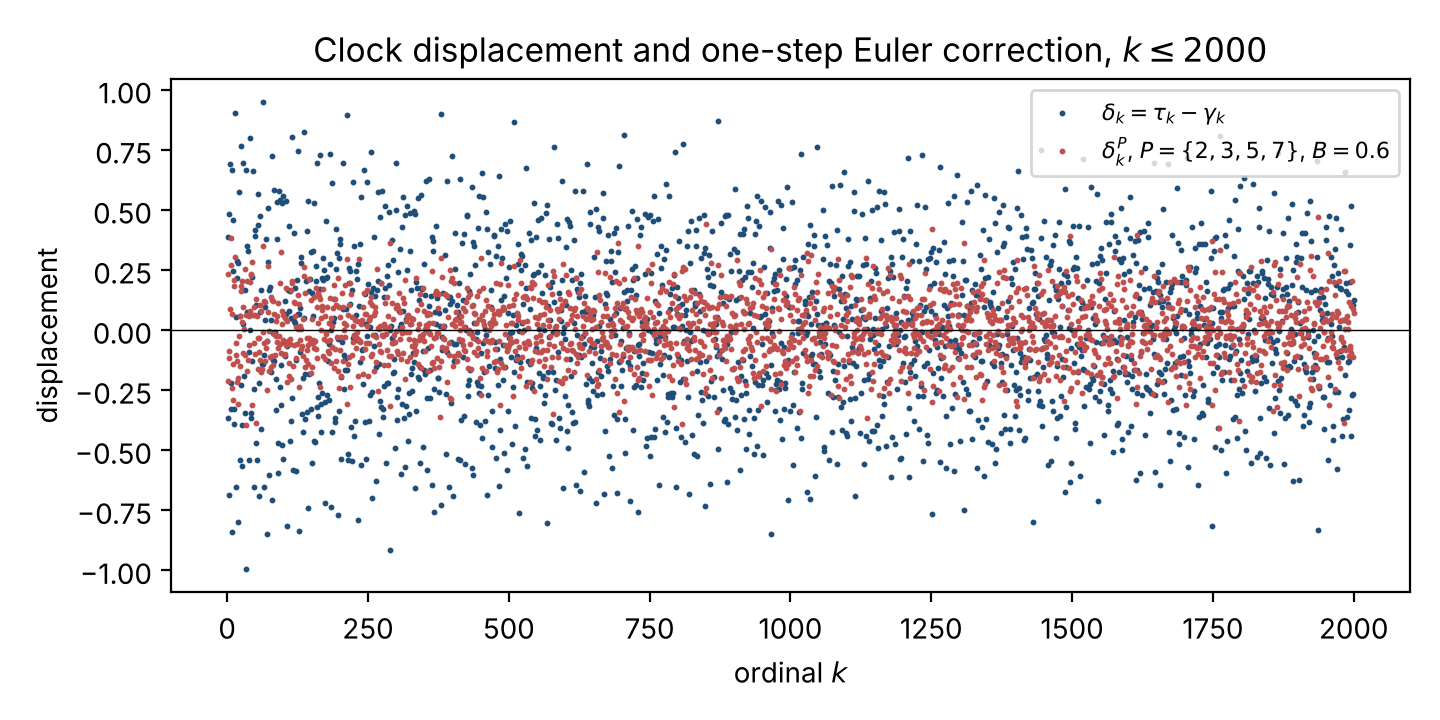
\includegraphics[width=0.85\textwidth]{fig01_displacement_first2000.png}
\caption{$\delta_k$ and the residual of the one-step clock with $P=\{2,3,5,7\}$, $\Omega=0.6$, for $k\le2000$.}
\label{fig:displacement}
\end{figure}

\begin{figure}[htbp]
\centering
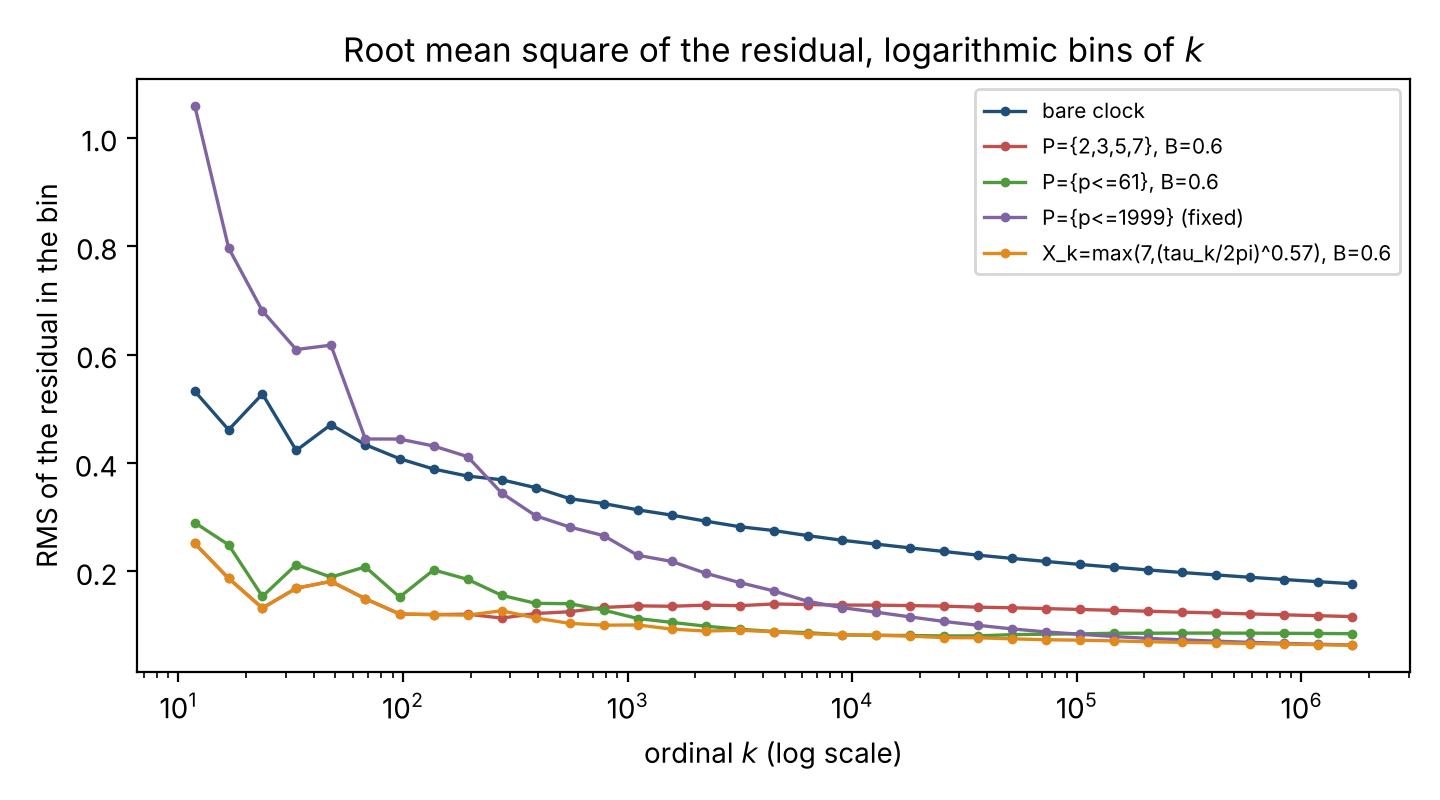
\includegraphics[width=0.85\textwidth]{fig02_rms_by_height.png}
\caption{RMS of the residual in logarithmic bins of $k$ (Experiment~\CGref{exp:methods}).}
\label{fig:rms_height}
\end{figure}

\begin{figure}[htbp]
\centering
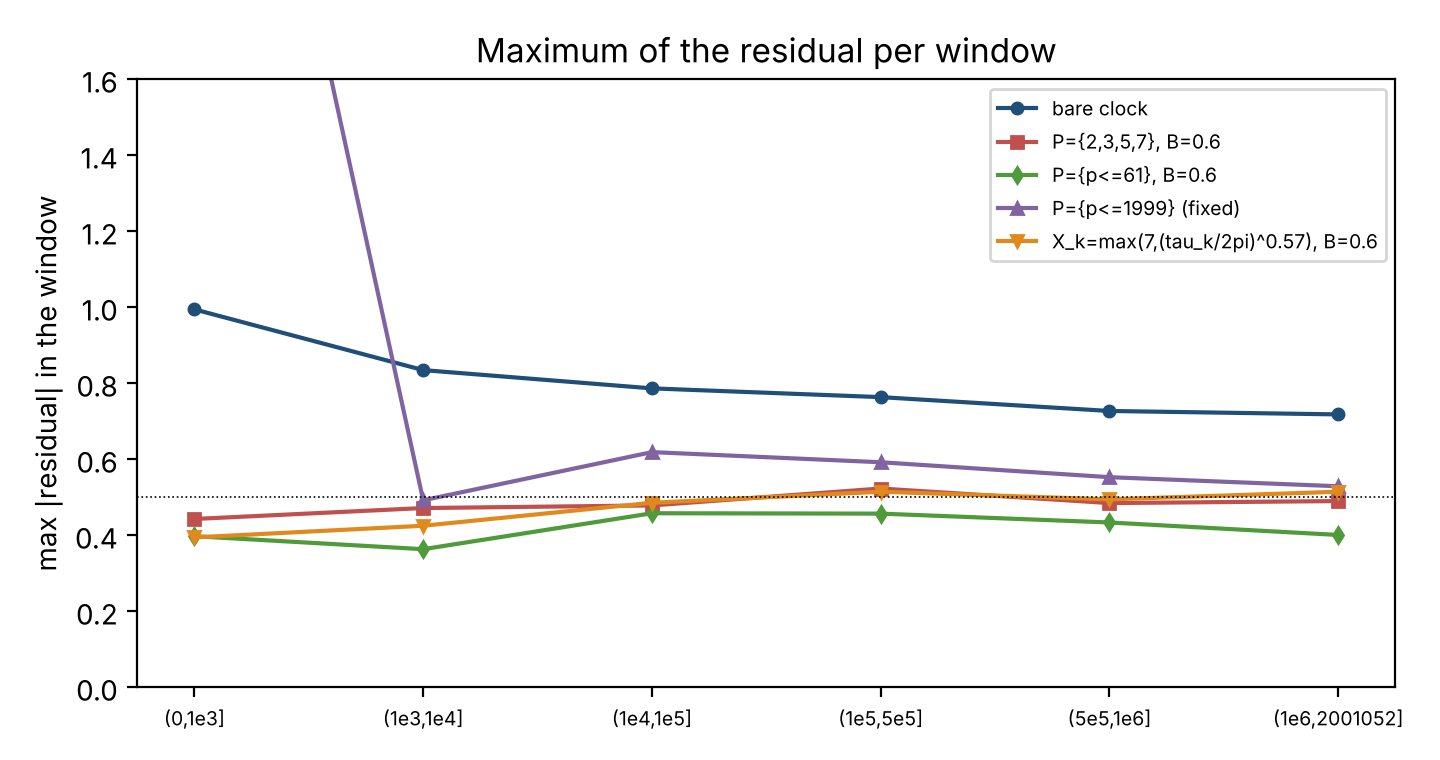
\includegraphics[width=0.85\textwidth]{fig08_max_by_window.png}
\caption{Maximum residual per window; dotted line $\frac12$ (Experiment~\CGref{exp:methods}).}
\label{fig:max_window}
\end{figure}

\begin{figure}[htbp]
\centering
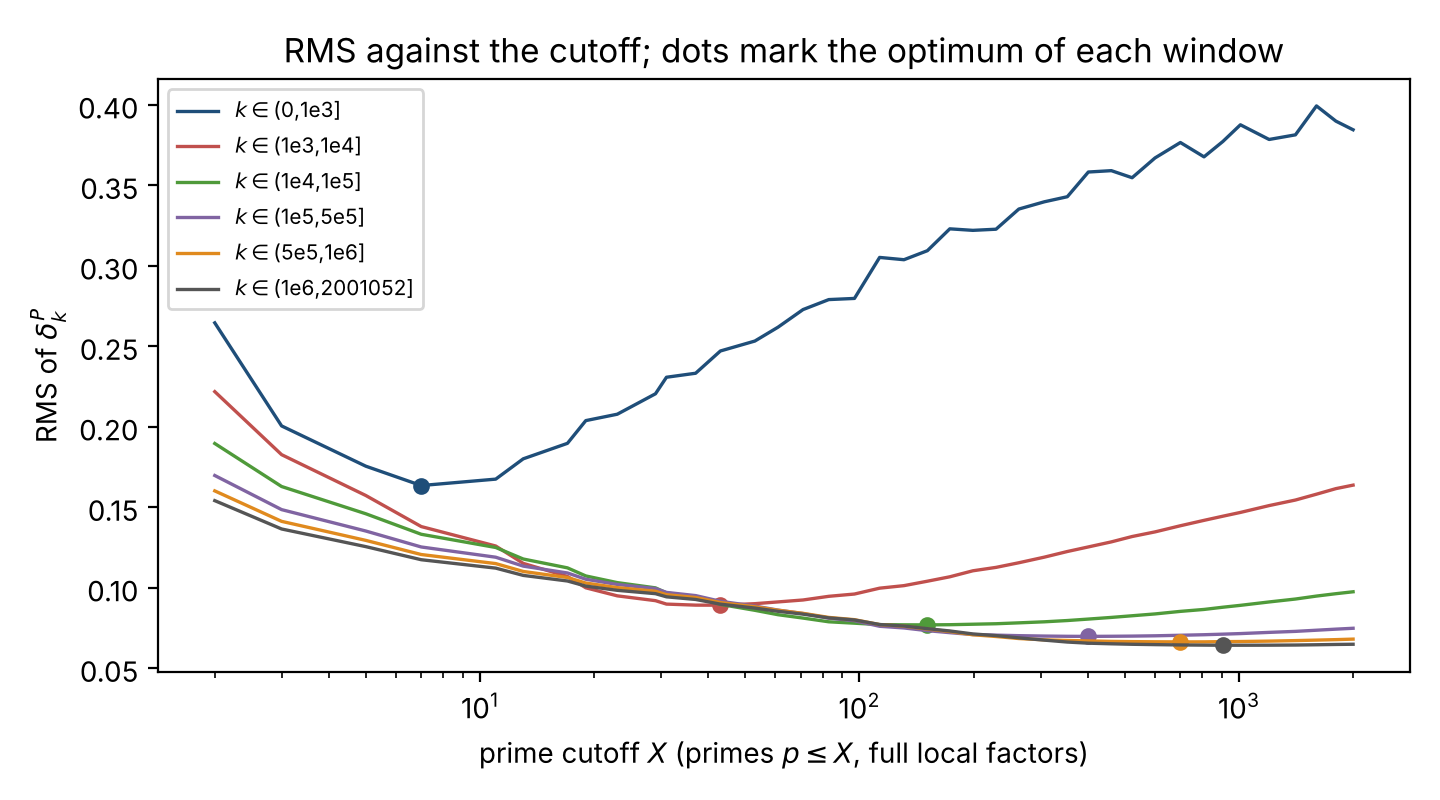
\includegraphics[width=0.85\textwidth]{fig03_rms_vs_cutoff.png}
\caption{RMS of the one-step residual against $X$ by window (Experiment~\CGref{exp:optimal_cutoff}).}
\label{fig:rms_cutoff}
\end{figure}

\begin{figure}[htbp]
\centering
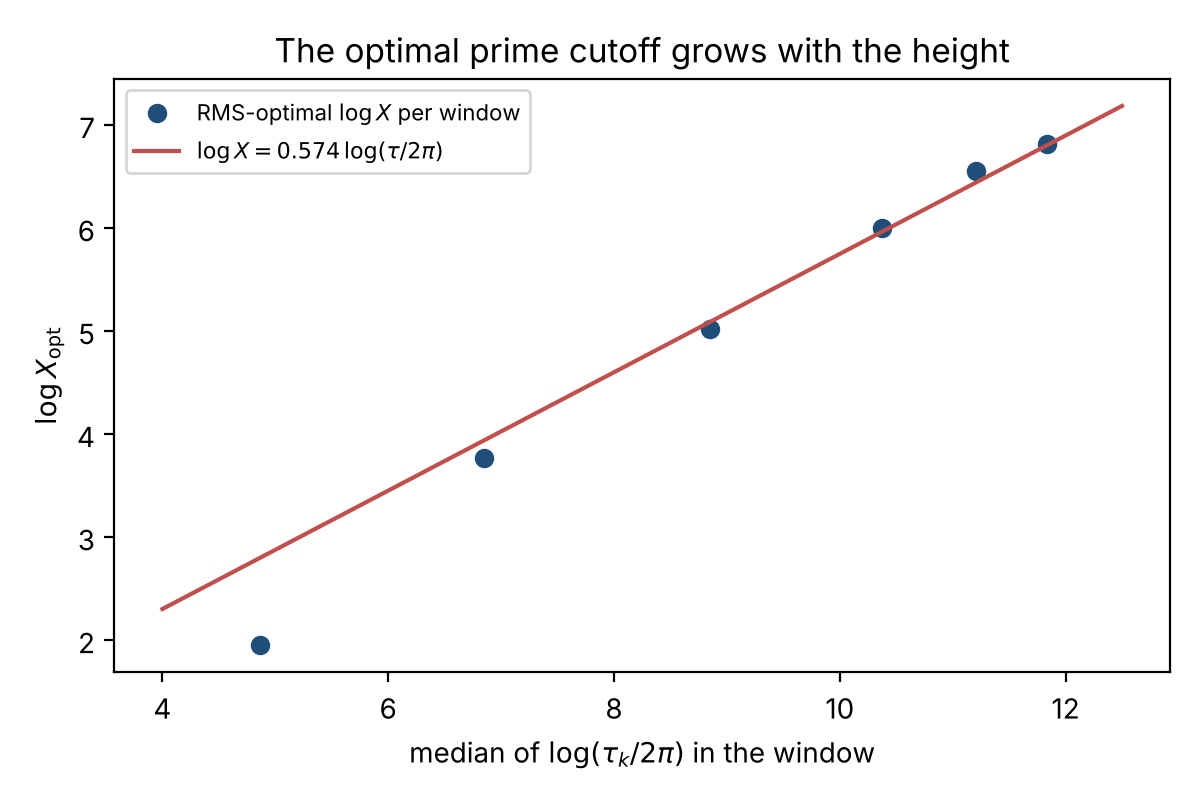
\includegraphics[width=0.65\textwidth]{fig04_optimal_cutoff.png}
\caption{Logarithm of the best scanned cutoff against the median of $\log(\tau_k/2\pi)$ (Experiment~\CGref{exp:optimal_cutoff}).}
\label{fig:optimal_cutoff}
\end{figure}

\begin{figure}[htbp]
\centering
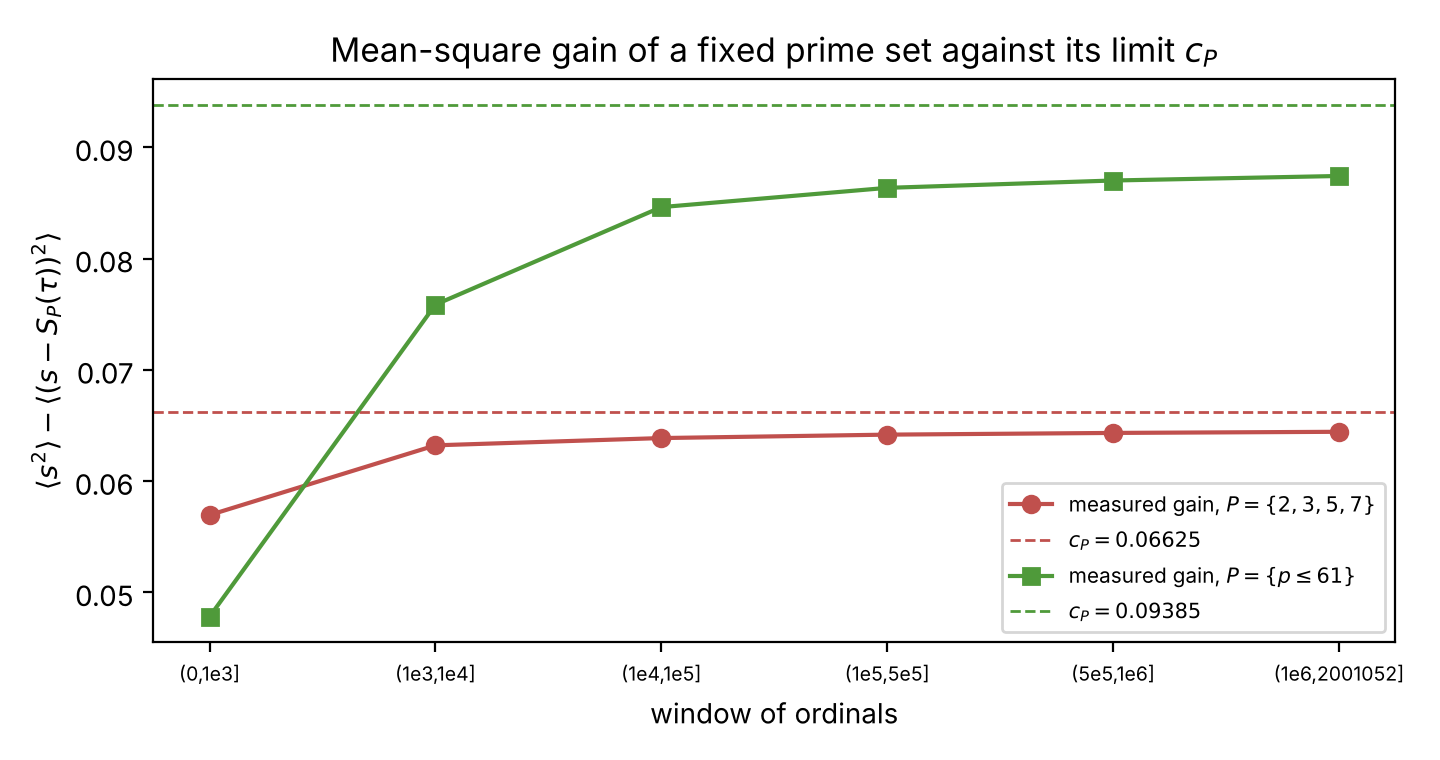
\includegraphics[width=0.85\textwidth]{fig07_gain_vs_theory.png}
\caption{Mean-square gain of fixed Euler phases and the constants $v^\infty_P$ (Experiment~\CGref{exp:gain}).}
\label{fig:gain}
\end{figure}

\begin{figure}[htbp]
\centering
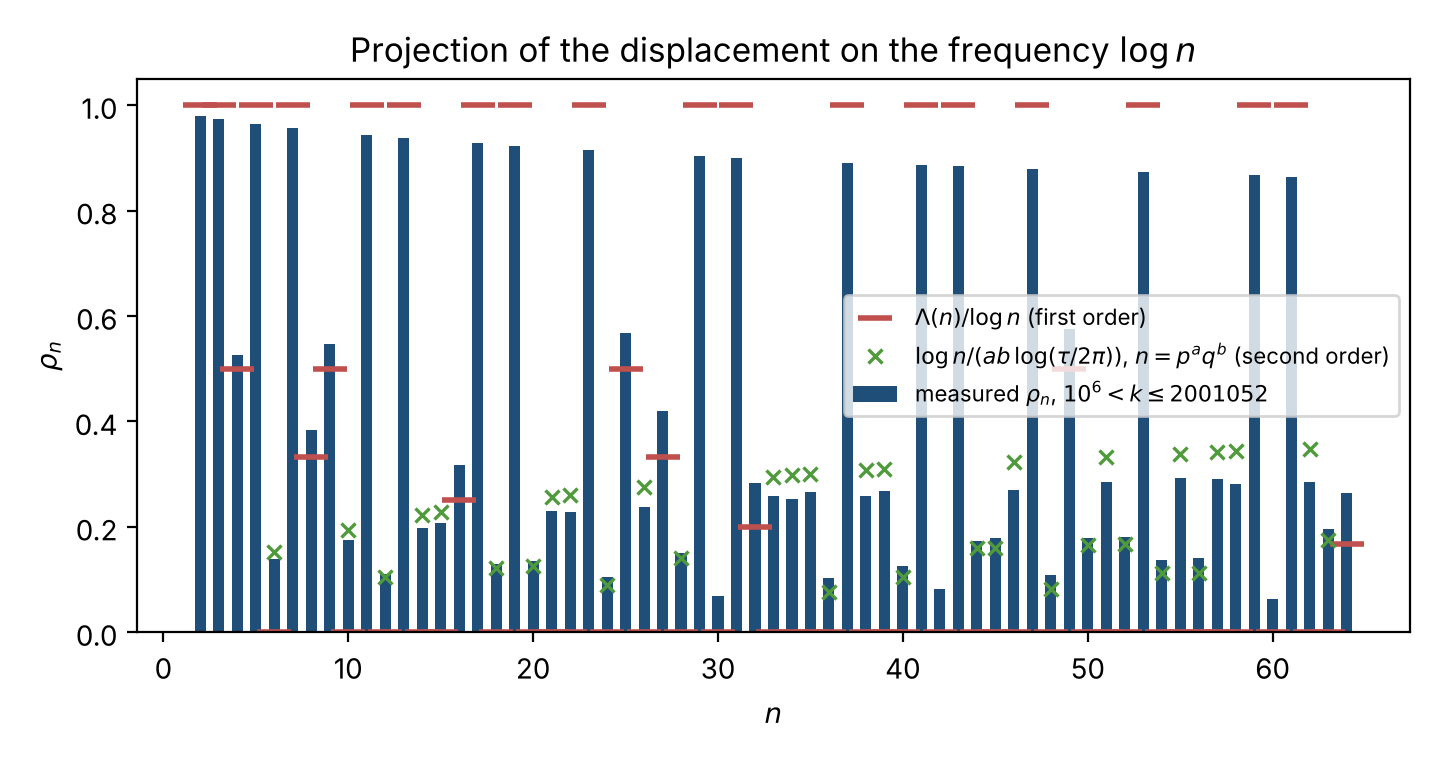
\includegraphics[width=0.85\textwidth]{fig05_projection_coefficients.png}
\caption{Projections $\rho_n$, $10^6<k\le K_*$ (Table~\CGref{tab:projection}).}
\label{fig:projection}
\end{figure}

\begin{figure}[htbp]
\centering
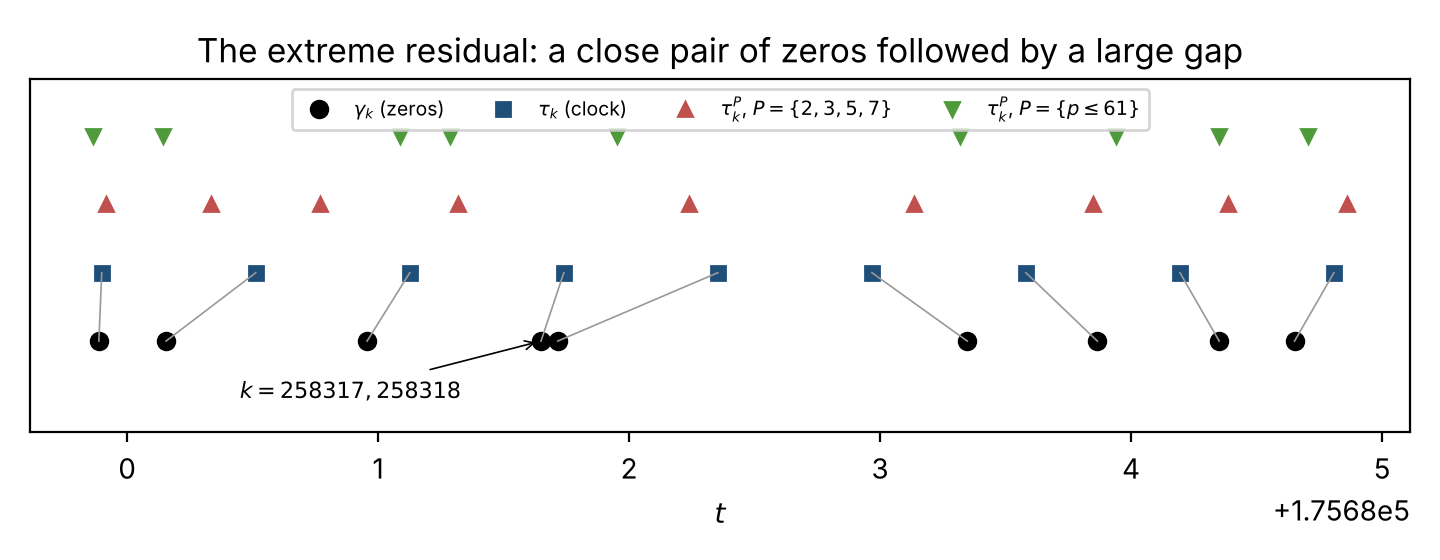
\includegraphics[width=0.85\textwidth]{fig06_close_pair.png}
\caption{Zeros, clock and one-step clocks around $k=258317,258318$ (Experiment~\CGref{exp:close_pair}).}
\label{fig:close_pair}
\end{figure}

\begin{figure}[htbp]
\centering
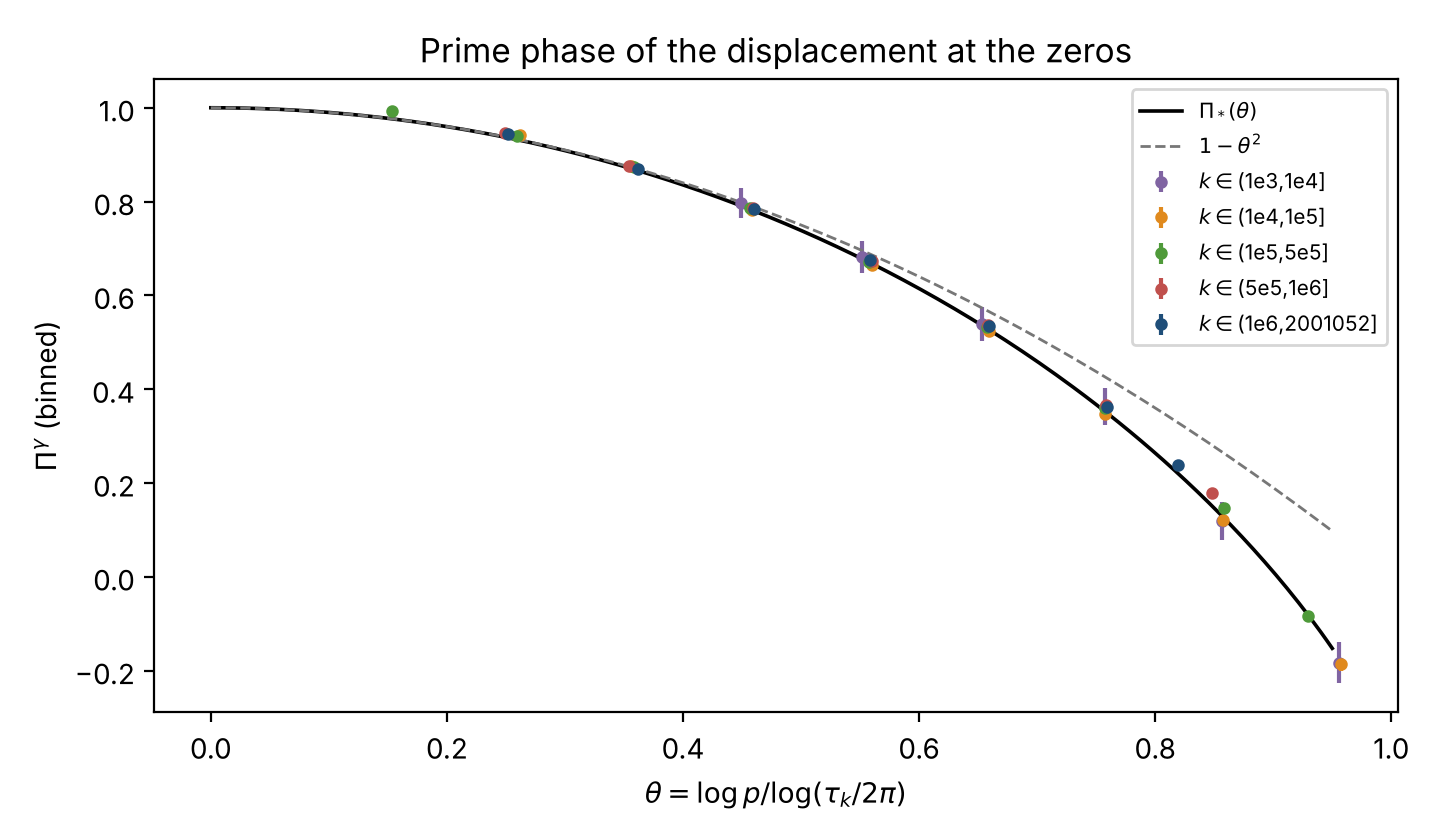
\includegraphics[width=0.85\textwidth]{fig09_phase_law.png}
\caption{Binned $\Pi^\gamma_p$ in five windows, the conjectured law $\Pi_*(\theta)$ and $1-\theta^2$ (Experiment~\CGref{exp:phase_law}).}
\label{fig:phase_law}
\end{figure}

\begin{figure}[htbp]
\centering
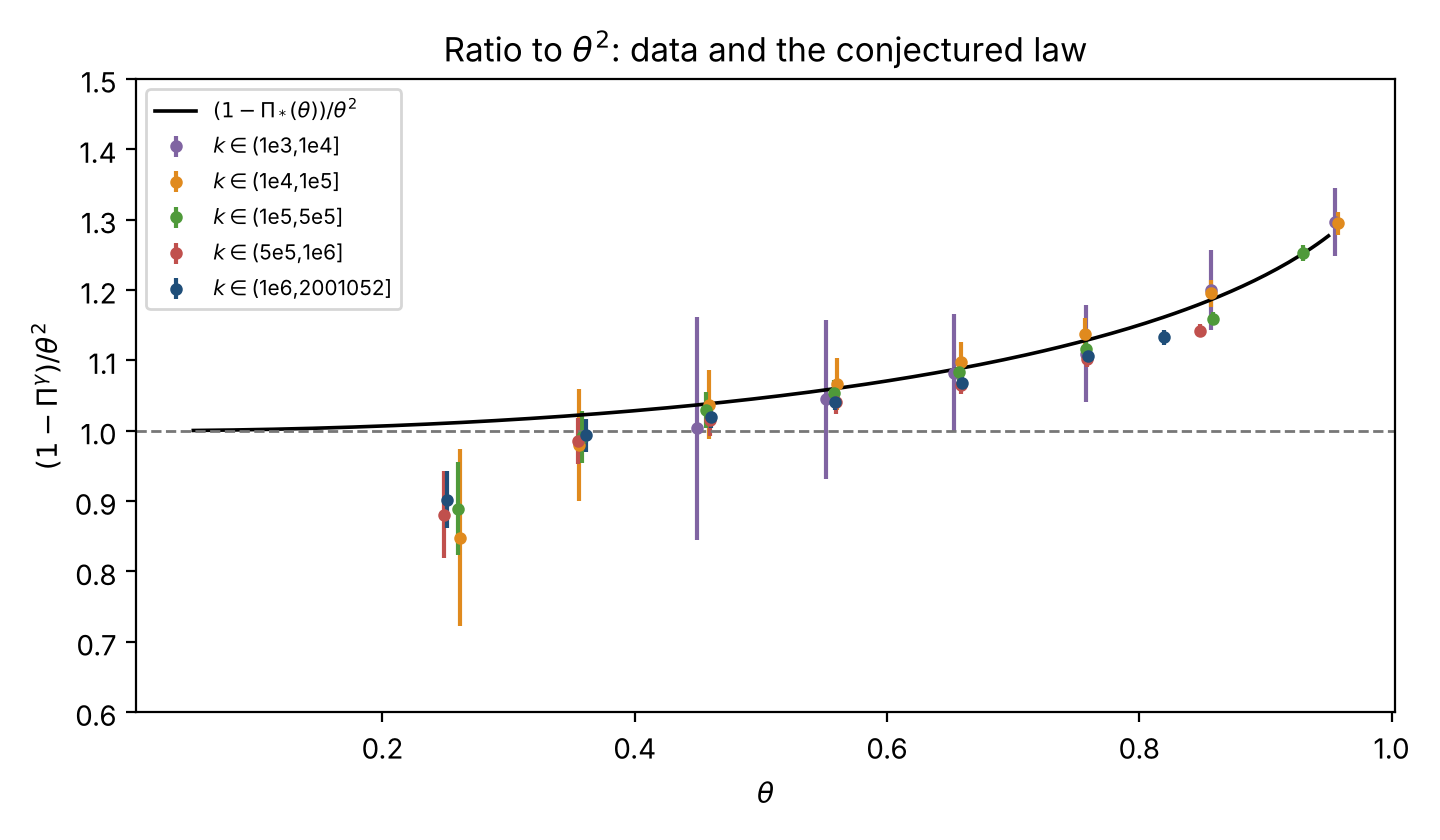
\includegraphics[width=0.85\textwidth]{fig10_phase_law_ratio.png}
\caption{$(1-\Pi^\gamma)/\theta^2$ with statistical errors and the conjectured ratio $(1-\Pi_*(\theta))/\theta^2$ (Experiment~\CGref{exp:phase_law}).}
\label{fig:phase_ratio}
\end{figure}

\begin{figure}[htbp]
\centering
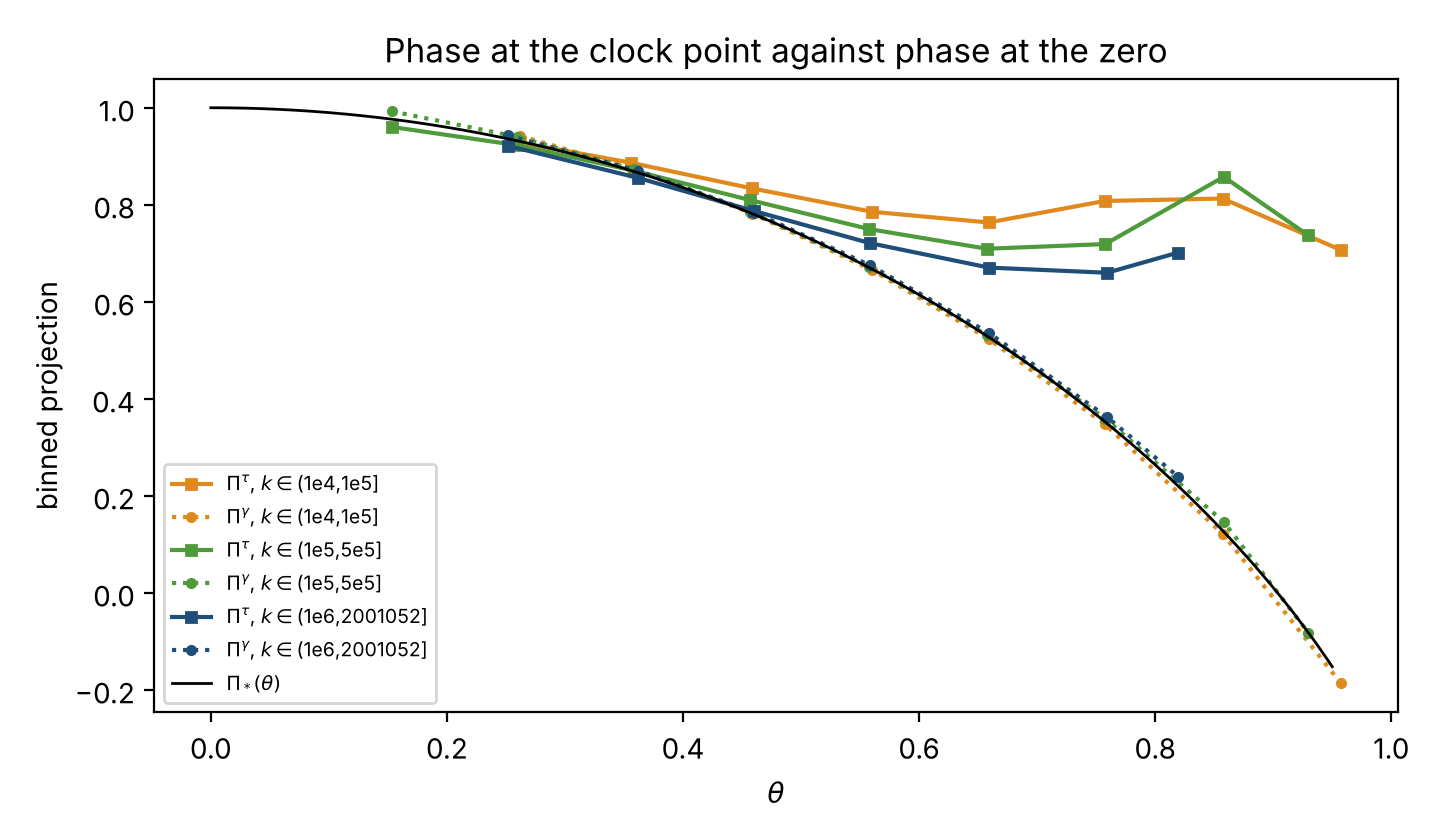
\includegraphics[width=0.85\textwidth]{fig11_phase_clock_vs_zero.png}
\caption{Binned $\Pi^\tau_p$ (clock) and $\Pi^\gamma_p$ (zero) in three windows (Experiment~\CGref{exp:phase_cos}).}
\label{fig:phase_clock}
\end{figure}

\section{Reproducibility}
\label{sec:reproducibility}
\texttt{code/opc\_analysis.py} produces Tables~\CGref{tab:methods}--\CGref{tab:close_pair}, \CGref{tab:scan_rms}--\CGref{tab:projection} and Figures~\CGref{fig:displacement}--\CGref{fig:close_pair} (about one minute); \texttt{code/opc\_phase\_law.py} produces Tables~\CGref{tab:accounting}, \CGref{tab:phase_law}--\CGref{tab:segment} and Figures~\CGref{fig:phase_law}--\CGref{fig:phase_clock} (about ten minutes). Both read \texttt{data/zeross.bin} and \texttt{data/zLamb.bin} ($K_*$ little-endian double-precision numbers each), which are not included in the repository because of their size; the second script checks their length and records their SHA-256 checksums. Both scripts are reproduced in Appendix~\CGref{sec:python_code}.

\section{Python code}
\label{sec:python_code}

\subsection{opc\_analysis.py}
\label{subsec:code_analysis}

@@CODE_ANALYSIS@@

\subsection{opc\_phase\_law.py}
\label{subsec:code_phase}

@@CODE_PHASE@@

\end{document}
